%%%%%%%%%%%%%%%%%%%%%%%%%%%%%%%%%%%%%%%%%%%%%%%%%
%%%%%%%%%%%% cap: Application design %%%%%%%%%%%%%%%%%
%%%%%%%%%%%%%%%%%%%%%%%%%%%%%%%%%%%%%%%%%%%%%%%%%
\chapter{Application Design}\label{cap:intro}

\section{Element of design}

\subsection{Introduction in design}

\hspace{\parindent}Application Design is an evolving field that leverages the principles of Design Theory and the practical approach of Design Thinking. It aims to strike a balance between form and function, aesthetics, and usability. \cite{fling2009mobile} This chapter will delve into the intricate application of these elements in creating interactive, effective, and visually appealing digital solutions, while also addressing the challenges faced during the process.
\hspace{\parindent}The task of designing applications is not a simple feat. It requires an understanding of the principles of Design Theory, such as balance, emphasis, rhythm, proportion, and unity. It also entails an in-depth comprehension of Design Thinking's core principles, including empathy for the user, the addition of solutions, and iterative refinement of designs.

\hspace{\parindent}Through this lens, Application Design transforms from a mere act of creating interfaces into a sophisticated process of solving problems and enhancing user experiences. This process requires both a strong foundation in theoretical principles and a human-centered approach that takes into account the context in which the application will be used.

\hspace{\parindent}In the scope of this chapter, we will dissect the core principles of Design Theory and Design Thinking and their respective roles in Application Design. We will illustrate how these principles and methods have been employed in real-world application design scenarios, underscoring their relevance and effectiveness. Furthermore, we also explore contemporary challenges and opportunities in Application Design, preparing readers to navigate and innovate in this ever-evolving field.

\hspace{\parindent}The chapter also elaborates on the iterative nature of Design Thinking and its inherent ability to learn from mistakes and progressively improve. We will discuss how Design Thinking and Application Design collectively ensure that digital solutions are not just functional but also user-centric.

\hspace{\parindent}In conclusion, this chapter will provide a comprehensive understanding of the symbiotic relationship between Design Theory, Design Thinking, and Application Design. The goal is to foster a robust theoretical and practical understanding that will enable designers to create applications that not only fulfill functional requirements but also resonate with users and deliver outstanding experiences.


Design theory is a broad and multifaceted field that encompasses many different areas of study, including graphic design, web design, user experience design, and more.  At its core, design theory is concerned with the principles and elements that underlie all forms of visual communication and problem-solving.
Design thinking is an essential component of design theory, and we will examine how this problem-solving approach is used in design to empathize with users, generate ideas, and iterate on solutions.

\subsection{Spacing}
The importance of maintaining constant spacing in design cannot be overstated. Consistent spacing, often referred to as spacing guidelines or whitespace management, plays a crucial role in enhancing the overall visual appeal and readability of a design. It ensures that elements are properly organized, allowing users to navigate and comprehend the content more effectively.

Spacing guidelines provide a sense of balance, harmony, and hierarchy within the design. By establishing consistent margins, padding, and line spacing, designers can create a cohesive and structured layout. This consistency helps users understand the relationships between different elements and makes the design more intuitive to navigate.

Proper spacing also contributes to the overall usability and accessibility of the design. Sufficient spacing between interactive elements, such as buttons or links, allows for easier selection and reduces the chance of accidental clicks. It enhances the user experience by providing a comfortable and uncluttered interface, which improves user satisfaction and engagement.

In addition, consistent spacing contributes to the perception of professionalism and attention to detail. It reflects a well-thought-out design process and gives the impression of a polished product. It shows that the designer has considered the overall user experience and visual aesthetics.

To maintain constant spacing, designers often establish grid systems or use design tools that provide layout guides and alignment features. This ensures that elements are aligned properly and follow the defined spacing guidelines consistently throughout the design.





\begin{enumerate}
  \item \textbf{Margins}: Maintain consistent margins around the edges of the design layout. This ensures that the content is not too close to the edges, providing breathing space and preventing visual clutter.
  
  \item \textbf{Padding}: Apply consistent padding within elements to create visual separation and prevent content from feeling cramped. This includes padding around text, images, buttons, and other interactive elements.
  
  \item \textbf{Line spacing}: Use line spacing in text blocks to improve readability. Ensure that lines of text are adequately spaced to avoid overcrowding or excessive gaps, making the content more visually appealing and easier to read.
  
  \item \textbf{Element spacing}: Maintain consistent spacing between elements such as buttons, icons, images, and paragraphs. This helps create a balanced and organized layout, allowing users to navigate and interact with the design more intuitively.
  
  \item \textbf{Grid systems}: Use grid systems to establish a consistent layout structure. Grids help align elements and maintain consistent spacing throughout the design, contributing to a visually pleasing and harmonious composition.
  
  \item \textbf{Responsive design}: Consider spacing guidelines for different screen sizes and devices. Optimize spacing to ensure that elements are properly proportioned and readable across various resolutions and orientations.
\end{enumerate}


\subsection{Grids}
Grid systems are a fundamental tool in design that provides a framework for organizing and aligning elements within a layout. They comprise a series of vertical and horizontal lines that create a structured grid of intersecting points or cells.

Grids offer several benefits in design:

\begin{enumerate}
  \item \textbf{Consistency and Structure}: Grids provide a consistent structure for organizing content, creating a sense of order and hierarchy. They help maintain visual consistency across different screens and pages within a project.
  
  \item \textbf{Alignment}: Grids facilitate the precise alignment of elements, ensuring that they are visually harmonious. By aligning elements to the grid, designers can achieve a more polished and professional look.
  
  \item \textbf{Proportional Layouts}: Grids enable designers to create proportional layouts by dividing the spacebar into well-defined columns and rows. This allows for more efficient use of space and helps maintain a balanced visual composition.
  
  \item \textbf{Flexibility and Responsiveness}: Grids can be designed to be flexible, allowing for fluid layouts that adapt to different screen sizes and orientations. By defining responsive breakpoints within the grid system, designers can ensure that the design remains cohesive and functional across various devices.
  
  \item \textbf{Efficiency and Workflow}: Grids provide a framework that streamlines the design process. They help designers make consistent decisions about spacing, sizing, and alignment, saving time and effort. Grid-based layouts also make it easier to maintain and update designs as the project evolves.
  
  \item \textbf{Visual Hierarchy}: Grids can establish a clear visual hierarchy within a design. By assigning different columns or rows different levels of importance, designers can guide the viewer’s attention and emphasize key elements.
\end{enumerate}

Grid systems can be customized to suit the specific needs of a project. They can vary in terms of column widths, gutter sizes, and the number of subdivisions. Designers can choose between fixed grids, where the columns and gutters have predefined sizes, or fluid grids, which adapt to the screen space.

By incorporating grid systems into their design process, designers can create layouts that are visually pleasing, organized, and easy to navigate. Grids serve as a foundational tool that supports the overall structure and coherence of a design, enhancing both the aesthetics and functionality of the final product.

To integrate grids in our application, we can define a grid system with a specific number of columns and spacing between them. By aligning elements to this grid, we can ensure consistency and proper organization.
\cite{webdesignres}
\begin{figure}[htbp]
  \centering
  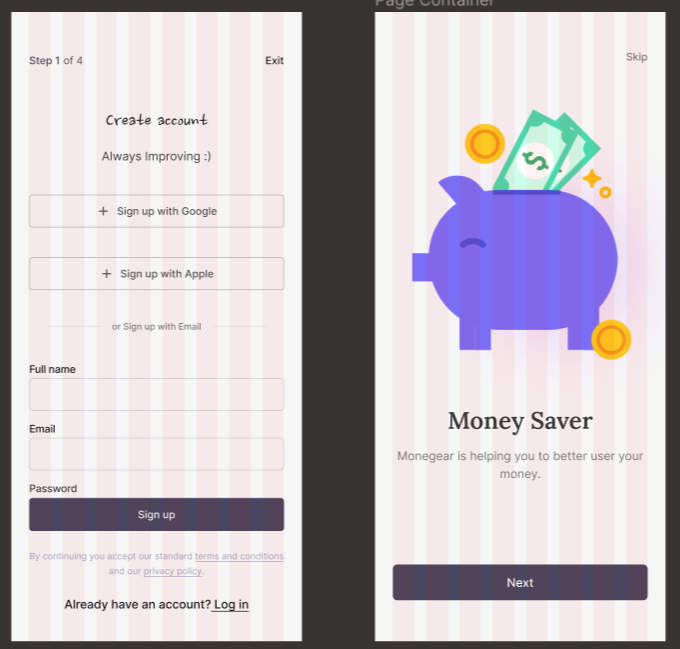
\includegraphics[width=0.8\textwidth]{Graphics/Design/Grids/image.png}
  \caption{Example of integrating grids in the application design}
  \label{fig:grid-example}
\end{figure}

In this example, we have implemented an 8-column grid system with a 4px baseline. The grid helps to align and structure various elements within the application's layout. Each column spans an equal width, and the baseline ensures consistent vertical spacing between elements.

By dividing the available space into eight columns, we create a proportional layout that can accommodate different components. The 4px baseline establishes a consistent vertical rhythm, ensuring that elements align harmoniously along the vertical axis.

The grid can guide the placement of elements such as text blocks, images, buttons, and other interactive components. By aligning these elements to the grid, we achieve a visually balanced and organized layout.

To ensure proper integration of the grid, designers can use design tools or frameworks that provide grid functionality. These tools assist in snapping elements to the grid and provide visual cues for aligning components accurately.

Integrating an 8-column, 4px baseline grid brings structure, consistency, and visual harmony to the application's design. It enhances readability, organization, and overall user experience. By following the grid guidelines, designers can create visually appealing and functional interfaces that resonate with users.




\subsection{Typography}
Typography is an essential element of design that encompasses the art and technique of arranging typefaces to create visually appealing and readable text. It plays a crucial role in various forms of communication, such as print media, digital interfaces, advertising, and branding.

At its core, typography is about selecting, organizing, and presenting typefaces in a deliberate and thoughtful manner. It involves making informed choices about font styles, sizes, spacing, alignment, and hierarchy to effectively convey information and evoke specific emotions or responses from the audience.

The primary goal of typography is to ensure readability and legibility. By choosing appropriate typefaces and adjusting factors like font size, line spacing, and letter spacing, typographers strive to create a text that is easy to read and comprehend. They consider the intended audience, context, and medium to optimize the reading experience.

Beyond readability, typography also plays a significant role in visual communication and aesthetics. It can evoke various moods, establish brand identities, and guide the viewer’s eye through a design. The arrangement of typefaces, hierarchy, and whitespace contribute to the overall visual impact and message of a piece.

Typography has a rich history dating back to the invention of movable type in the 15th century, which revolutionized printing and led to the proliferation of books. Over the centuries, typographic styles and practices have evolved, reflecting cultural shifts, artistic movements, and technological advancements.

In the digital age, typography has become even more versatile and accessible. Designers can choose from an extensive range of typefaces, customize them with digital tools, and experiment with dynamic and interactive typography in digital interfaces.

Understanding the principles and techniques of typography empowers designers to effectively communicate through text. By employing typography thoughtfully, they can enhance readability, express ideas, evoke emotions, and create visually engaging designs that capture and hold the viewer’s attention.

In this chapter, we will explore the fundamental principles, best practices, and practical applications of typography in [specify the context of your paper]. Through this exploration, we aim to show the significance of typography in design and its impact on effective visual communication.




\begin{itemize}
  \item \textbf{Font Selection}: Carefully selecting appropriate fonts that align with the purpose and tone of your paper while considering factors such as readability, professionalism, and brand consistency.
  
  \item \textbf{Hierarchy}: Establishing a clear visual hierarchy within the typography to guide readers' attention and emphasize key points. This can be achieved through variations in font sizes, weights, and styles, ensuring that important information stands out.
  
  \item \textbf{Readability}: Ensuring that the text is easily readable by selecting suitable font sizes, line spacing, and letter spacing. Avoiding overcrowding of text and choosing legible typefaces contribute to the overall readability of your paper.
  
  \item \textbf{Alignment}: Employing proper text alignment, such as left-aligned or justified, to enhance readability and maintain a polished appearance throughout the paper. Consistency in alignment creates a cohesive and visually pleasing reading experience.
  
  \item \textbf{Whitespace}: Using whitespace effectively to provide visual breathing space between elements and enhance overall clarity. Proper use of whitespace contributes to improved readability and helps organize content in a balanced manner.
  
  \item \textbf{Consistency}: Maintaining consistency in typography throughout your paper by using consistent font choices, sizes, styles, and alignment. Consistency creates a cohesive visual identity and fosters a professional appearance.
  
  \item \textbf{Brand Identity}: Using typography to reflect and reinforce your paper's brand identity or academic institution. Selecting fonts that align with the overall style and values of your paper can create a consistent and recognizable visual identity.
  
  \item \textbf{Visual Impact}: Employing creative typographic treatments, such as emphasis through bold or italicized text, varying font sizes for headings, or using typographic hierarchy to create visual interest and impact in your paper.
  
  \item \textbf{Effective Communication}: Leveraging typography to enhance the communication of information in your paper. By employing proper font choices, alignment, and hierarchy, you can effectively convey your research findings and ideas to your readers.
\end{itemize}




\begin{figure}[htbp]
  \centering
  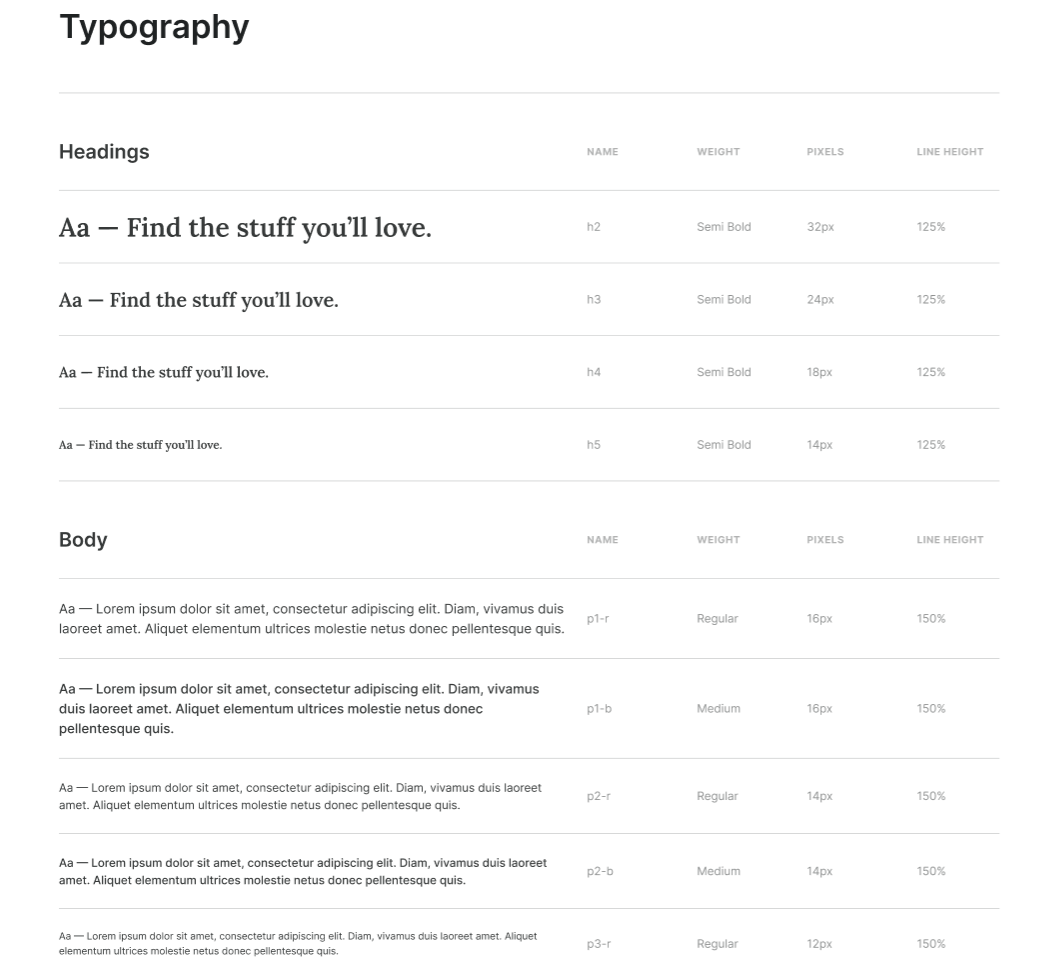
\includegraphics[width=0.5\textwidth]{Graphics/Design/Typograpghty/image.png}
  \caption{Typography template}
  \cite{fling2009mobile}
\end{figure}




\subsection{Color}

Color is a fundamental element of design that holds immense significance in conveying messages, evoking emotions, and creating visual interest. It is a powerful tool that can capture attention, establish a visual hierarchy, and elevate the overall user experience. Designers meticulously consider various aspects when working with color to ensure their designs effectively communicate their intended message and captivate their audience.

The color goes beyond its visual appeal. It possesses the ability to evoke emotions, create associations, and convey meaning. Designers delve into the psychology of color, understanding the psychological responses that different colors elicit in individuals. They explore the emotional impact of colors and handpick hues that align with their desired emotional response and convey their intended message effectively.

\begin{enumerate}
\item \textbf{Psychology of Color}: Designers consider the psychological associations and emotional responses associated with different colors. By understanding the psychology of color, designers can select colors that align with their intended message and evoke the desired emotions in their audience.

\item \textbf{Color Harmony}: Achieving color harmony involves selecting colors that complement each other and create a visually pleasing composition. Designers carefully choose color combinations that work well together, ensuring a balanced and harmonious visual experience.

\item \textbf{Contrast}: Contrast is an essential consideration in color selection. Designers use contrast to create visual interest, distinguish important elements, and improve readability. By carefully balancing colors with different levels of contrast, designers ensure that key information stands out effectively.

\item \textbf{Color Symbolism}: Colors carry symbolic meanings that can vary across cultures and contexts. Designers consider the cultural connotations associated with different colors to ensure their choices align with the intended message and avoid any potential misinterpretation or conflicts.

\item \textbf{Color Accessibility}: Designers prioritize color accessibility by considering the needs of all users, including those with visual impairments or color blindness. They ensure sufficient color contrast for readability and provide alternative means of conveying information beyond color alone.

\item \textbf{Color Consistency}: Consistency in color usage helps establish a strong visual identity and brand recognition. Designers define a color palette and adhere to it consistently, ensuring that colors remain cohesive across various touch points and materials.

\item \textbf{Color and User Experience}: Colors significantly impact the user experience. Designers leverage color to influence users' perception of usability, credibility, and enjoyment. By employing colors strategically, designers create engaging and intuitive experiences for their audience.

\item \textbf{Color Trends and Brand Differentiation}: Designers stay informed about color trends to create contemporary and visually appealing designs. They also consider unique color choices or combinations to differentiate their brand or product from competitors, fostering brand recognition and recall.
\end{enumerate}

\begin{figure}[htbp]
  \centering
  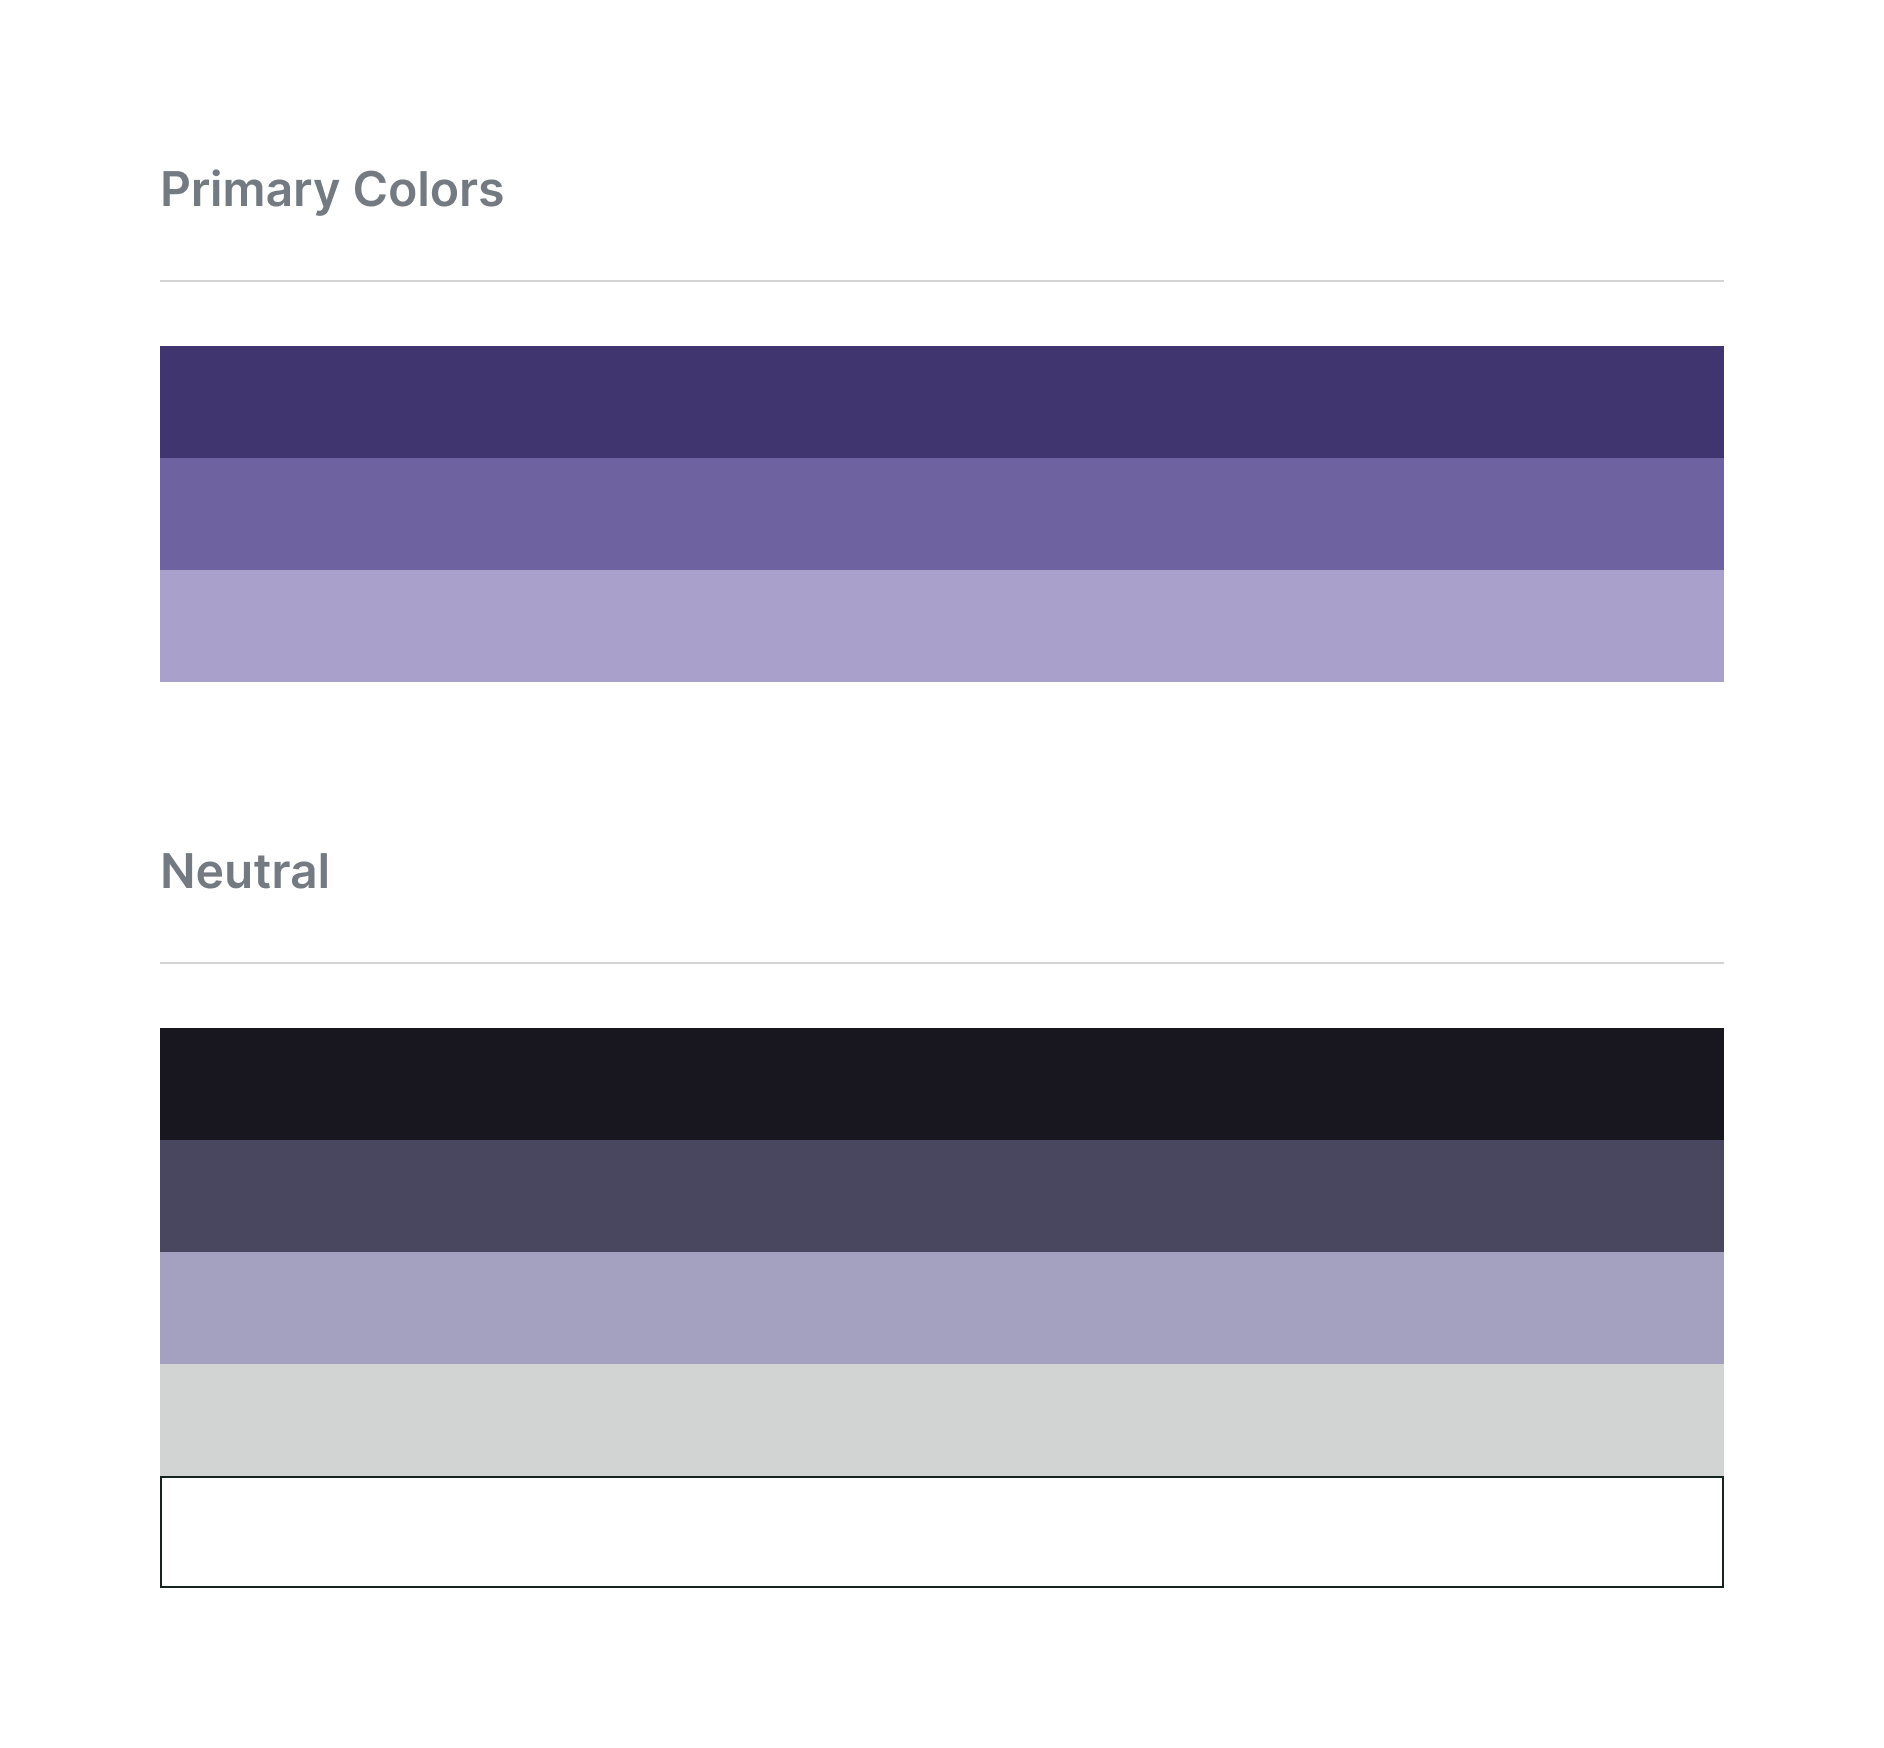
\includegraphics[width=0.5\textwidth]{Graphics/Design/Color Pallet.png}
  \caption{Typography template}
\end{figure}




\section{Design choices}\label{sect:description}


\hspace{\parindent}The design of the Moneager application was approved Development
3.1 Database Structure
3.2 Endpoints (GraphQL)
19
ched with the user in mind, aiming to create an intuitive and visually pleasing experience. The following design principles were taken into consideration during the development process:

\hspace{\parindent} \textbf{Simplicity}: The application was designed to be as simple and user-friendly as possible, with a clean and uncluttered layout. This allows users to easily navigate the app and access the features they need without feeling overwhelmed.

\hspace{\parindent} \textbf{Consistency}: The visual elements and design patterns used throughout the application are consistent, creating a cohesive and recognizable user interface. This enhances the user experience by reducing confusion and cognitive load.

\hspace{\parindent} \textbf{Usability}: The user interface was designed to be intuitive and easy to use, with clear navigation and visual cues to guide the user. The goal was to create an application that can be used by anyone, regardless of their level of technical expertise.

\hspace{\parindent}\textbf{Visual Appeal:} The application was designed with a modern and visually appealing layout, using a consistent color scheme and typography to create a polished and professional look. This was done to ensure that users enjoy using the application and are motivated to continue using it.

\hspace{\parindent}In terms of specific design decisions, the application features a minimalistic design with a focus on usability. The layout is centered around the main menu, which provides easy access to all of the application's features. The use of icons and visual elements is consistent throughout the application, enhancing the user experience by making it easy to recognize and navigate different sections of the app.


\hspace{\parindent}Another design choice is the use of a modern and sleek layout with a balanced amount of features to ensure simplicity and ease of use for all users. The use of a simple and intuitive navigation system, with clear visual elements and typography, is also prioritized to enhance user experience. Additionally, the incorporation of a high-contrast option and alternative text for images ensures accessibility for all users.

\hspace{\parindent}Overall, the design choices made for the Moneager application were focused on creating a user-friendly and visually appealing experience, with a balance between simplicity and functionality.\




\hspace{\parindent}Design choices are crucial for any mobile application, especially for a financial management application that requires users to engage with the app frequently. One of the primary design choices for this application is the elimination of a drawer menu, which can often clutter the user interface and make navigation confusing. Instead, a user-friendly bottom tab navigation system is implemented to ensure ease of use and simplify the user interface.

\hspace{\parindent}The design layout of the application has been carefully crafted to ensure a modern and minimalistic look, while still providing users with the necessary features to manage their finances efficiently. The use of a clean and consistent layout with adequate white space and appropriate visual elements is crucial for a user-friendly interface. This design ensures that users can easily navigate the application and find the information they need quickly and efficiently.




\hspace{\parindent} First of all the design is quite a complex step so I tried to iterate multiple designs. 
In the next Subsection I will describe my design motivation for this design and what are reasons why I had not continued with it.

\subsection{First Design Iteration}

When selecting colors for different transaction types in the application, a set of guidelines and considerations were followed. The primary aim was to ensure that the chosen colors were easily distinguishable. The colors were selected based on their association with the corresponding transaction types commonly recognized by users.

In the color selection for different transaction types in the application, the following associations were made:

Certainly! Here's the information presented in a list format using LaTeX code:

\begin{itemize}
  \item Income transactions: \textbf{Green} - commonly associated with money and growth.
  \item Expenses: \textbf{Red} - chosen due to its association with negative actions or consequences.
  \item Investing: \textbf{Yellow} or \textbf{gold} - symbolizing wealth and luxury.
  \item Savings: \textbf{Blue} - selected for its connotations of stability and reliability.
\end{itemize}


These color choices were made to ensure easy distinguishing ability and to align with the recognized associations of these colors by users.

It is important to note that, during the color selection process, the goal was to create a visually balanced composition that would enhance the application's overall usability and modernity. The chosen colors were carefully implemented to maintain simplicity while incorporating enough features. The resulting design layout, illustrated in the accompanying Figma file, showcases the successful execution of these principles.

Upon reflection, it was realized that some color compositions were uneven and required further changes to ensure a harmonious visual presentation.

\hspace{\parindent}Below, we provide some illustrations that showcase the design layout of the application. The illustrations demonstrate how the application has been developed to prioritize simplicity, usability, and modernity, with a balanced amount of features and a sleek design.

\begin{figure}[htbp]
  \centering
  \begin{minipage}[b]{0.32\textwidth}
    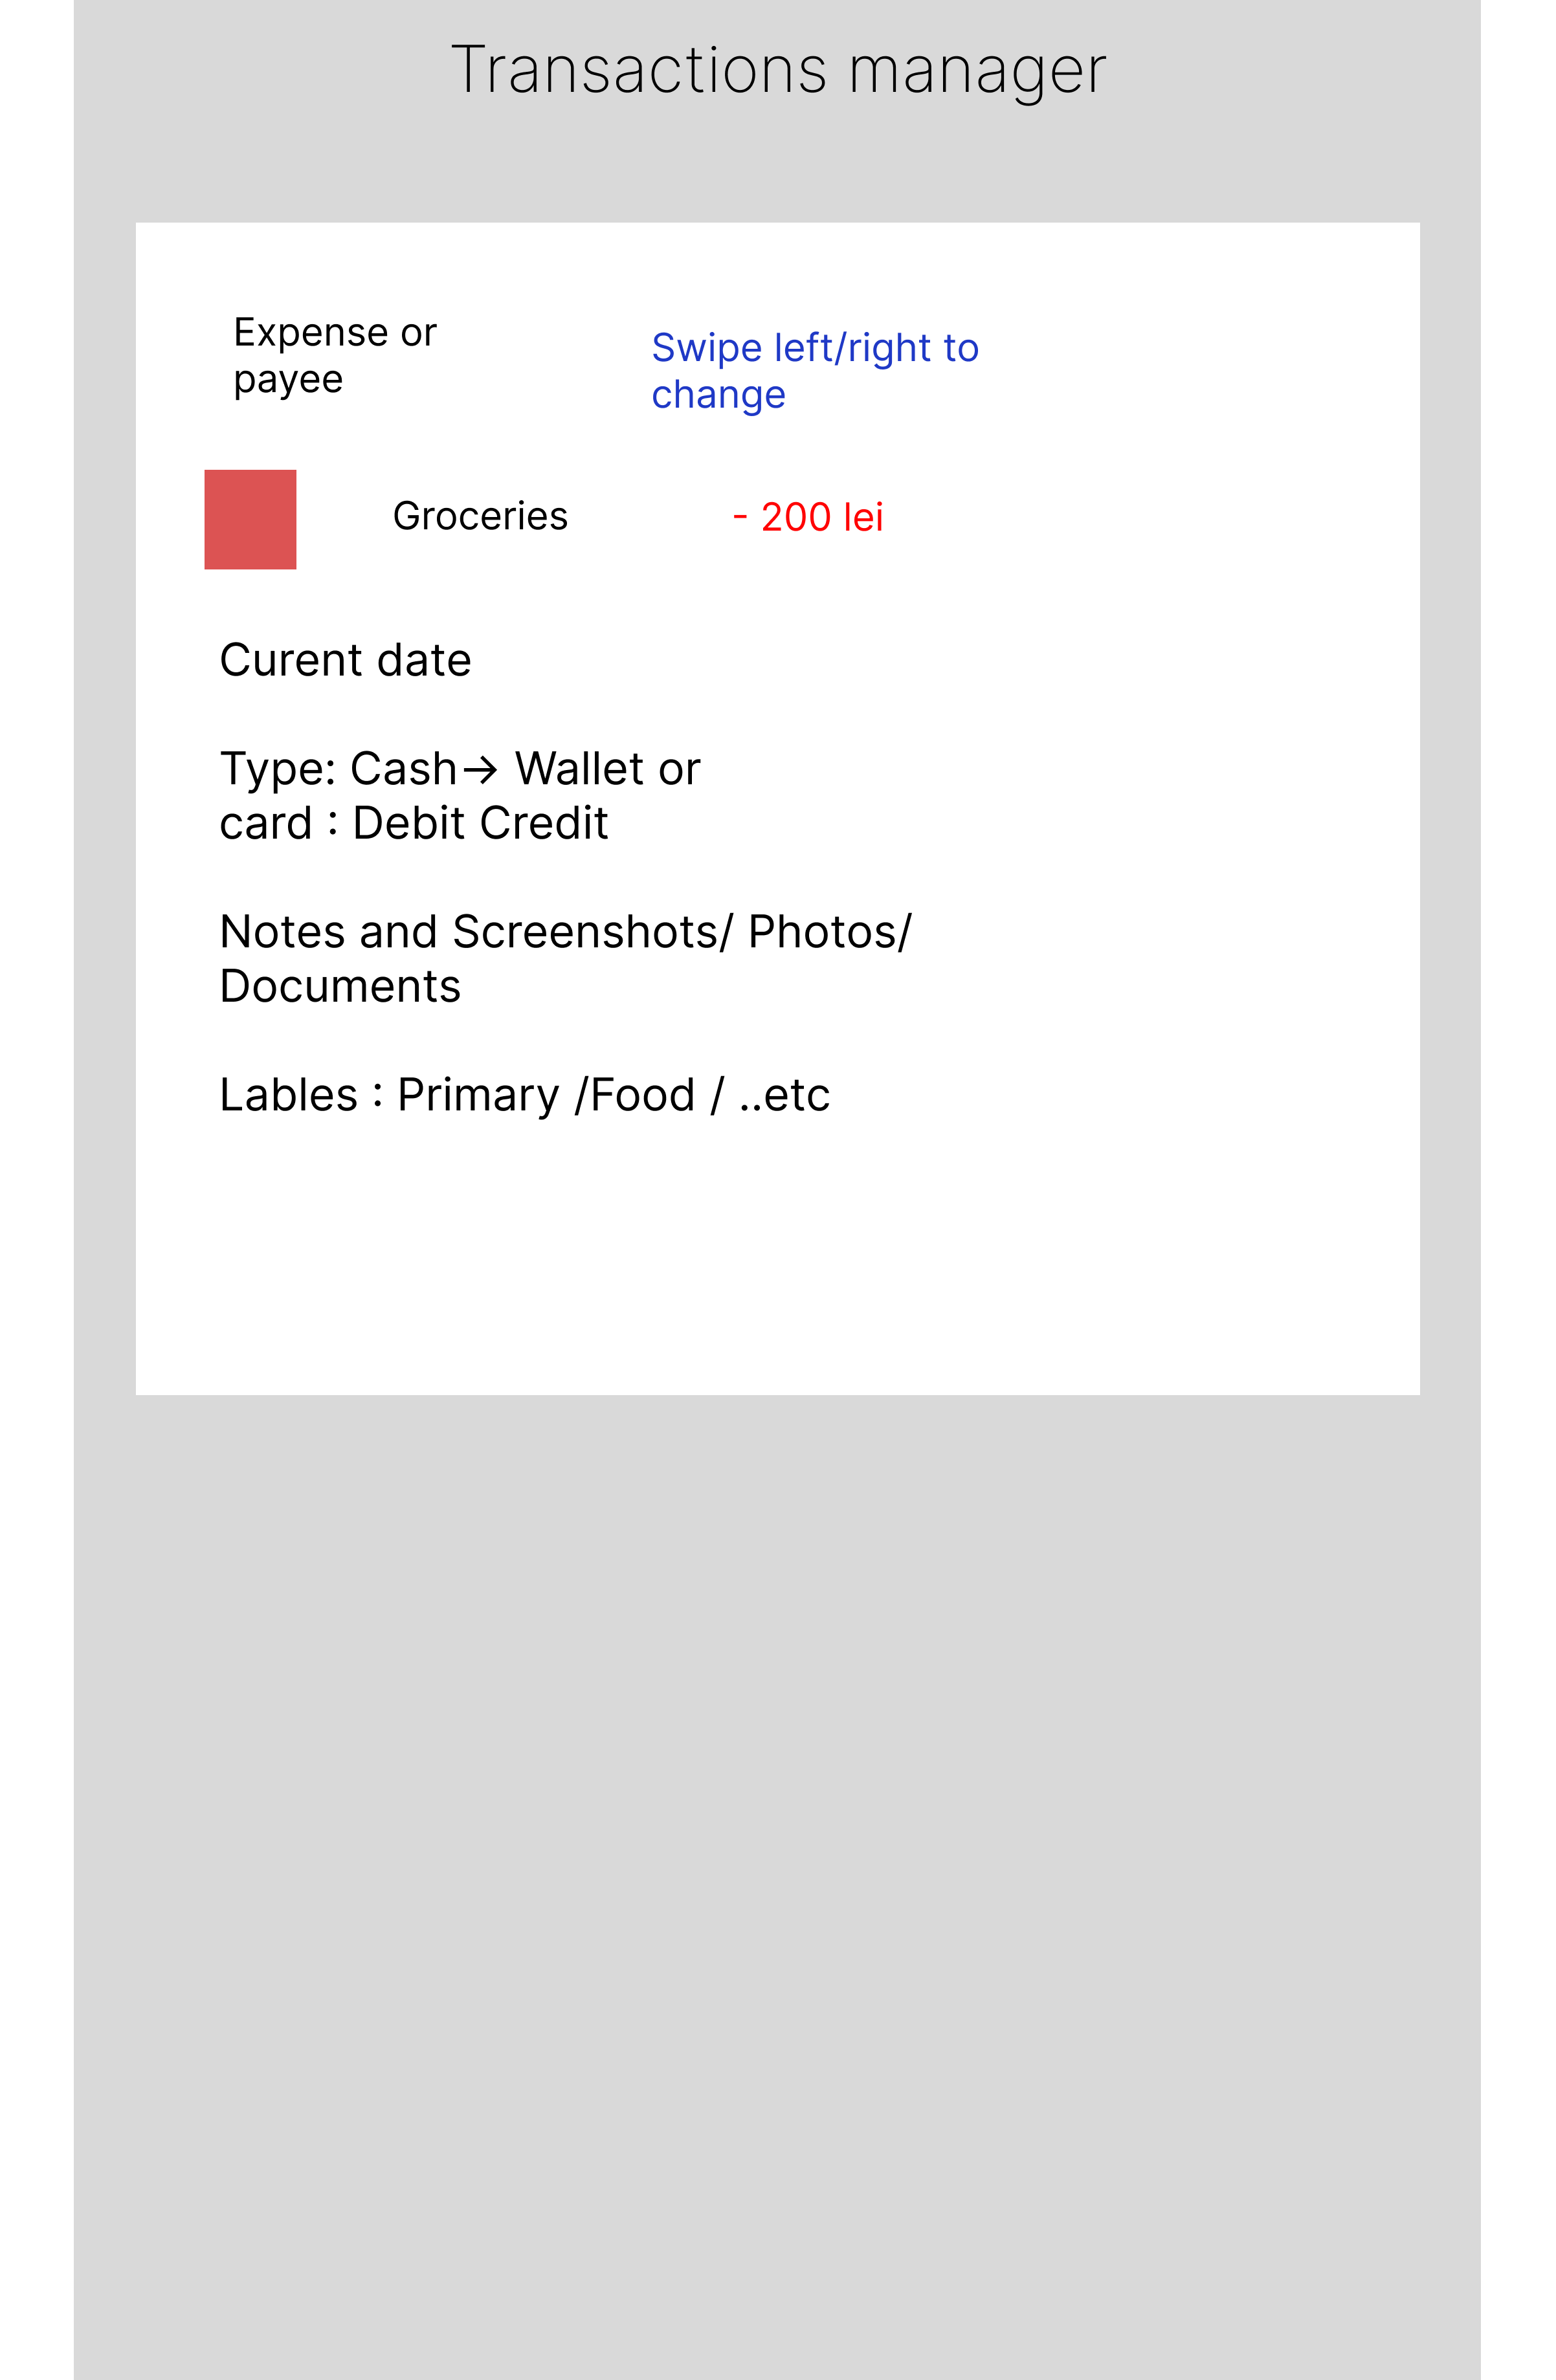
\includegraphics[width=\textwidth]{Graphics/Design/TM_E.png}
    \caption{Expense Transaction Screen}
    \label{fig:image1}
  \end{minipage}
  \hfill
  \begin{minipage}[b]{0.32\textwidth}
    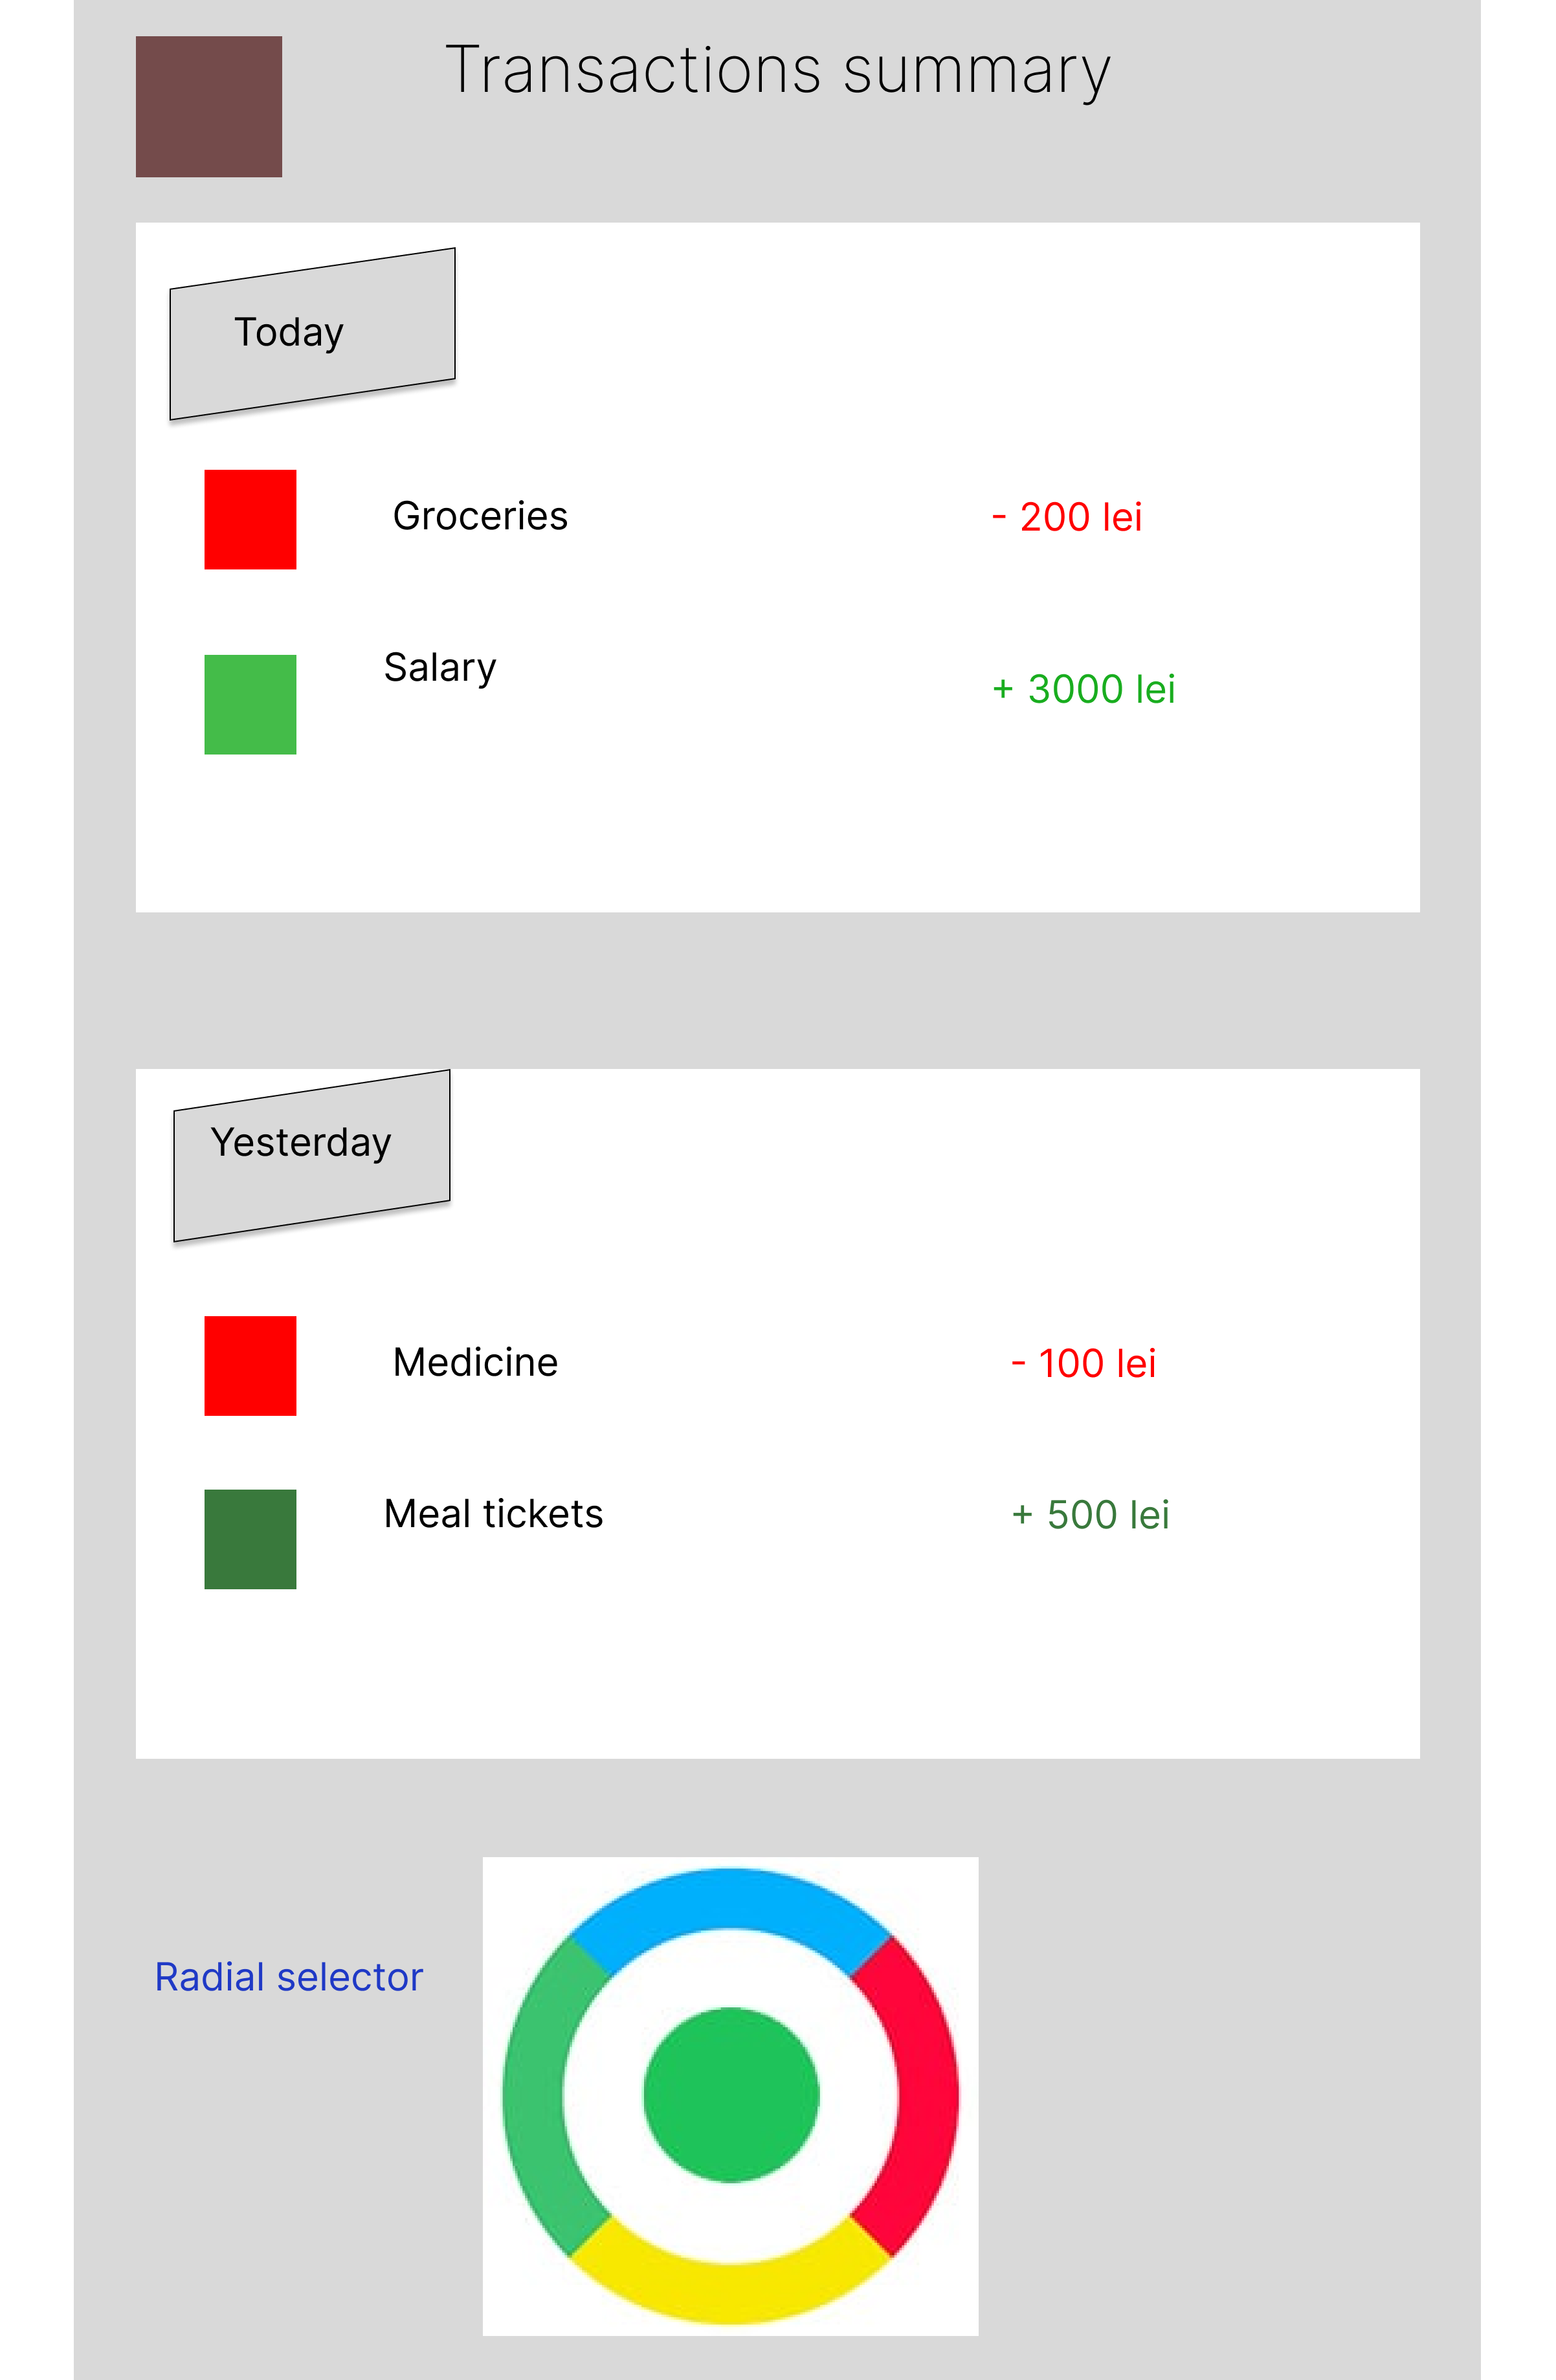
\includegraphics[width=\textwidth]{Graphics/Design/TM_Menu.png }
    \caption{Transaction Creator Menu}
    \label{fig:image2}
  \end{minipage}
  \hfill
  \begin{minipage}[b]{0.32\textwidth}
    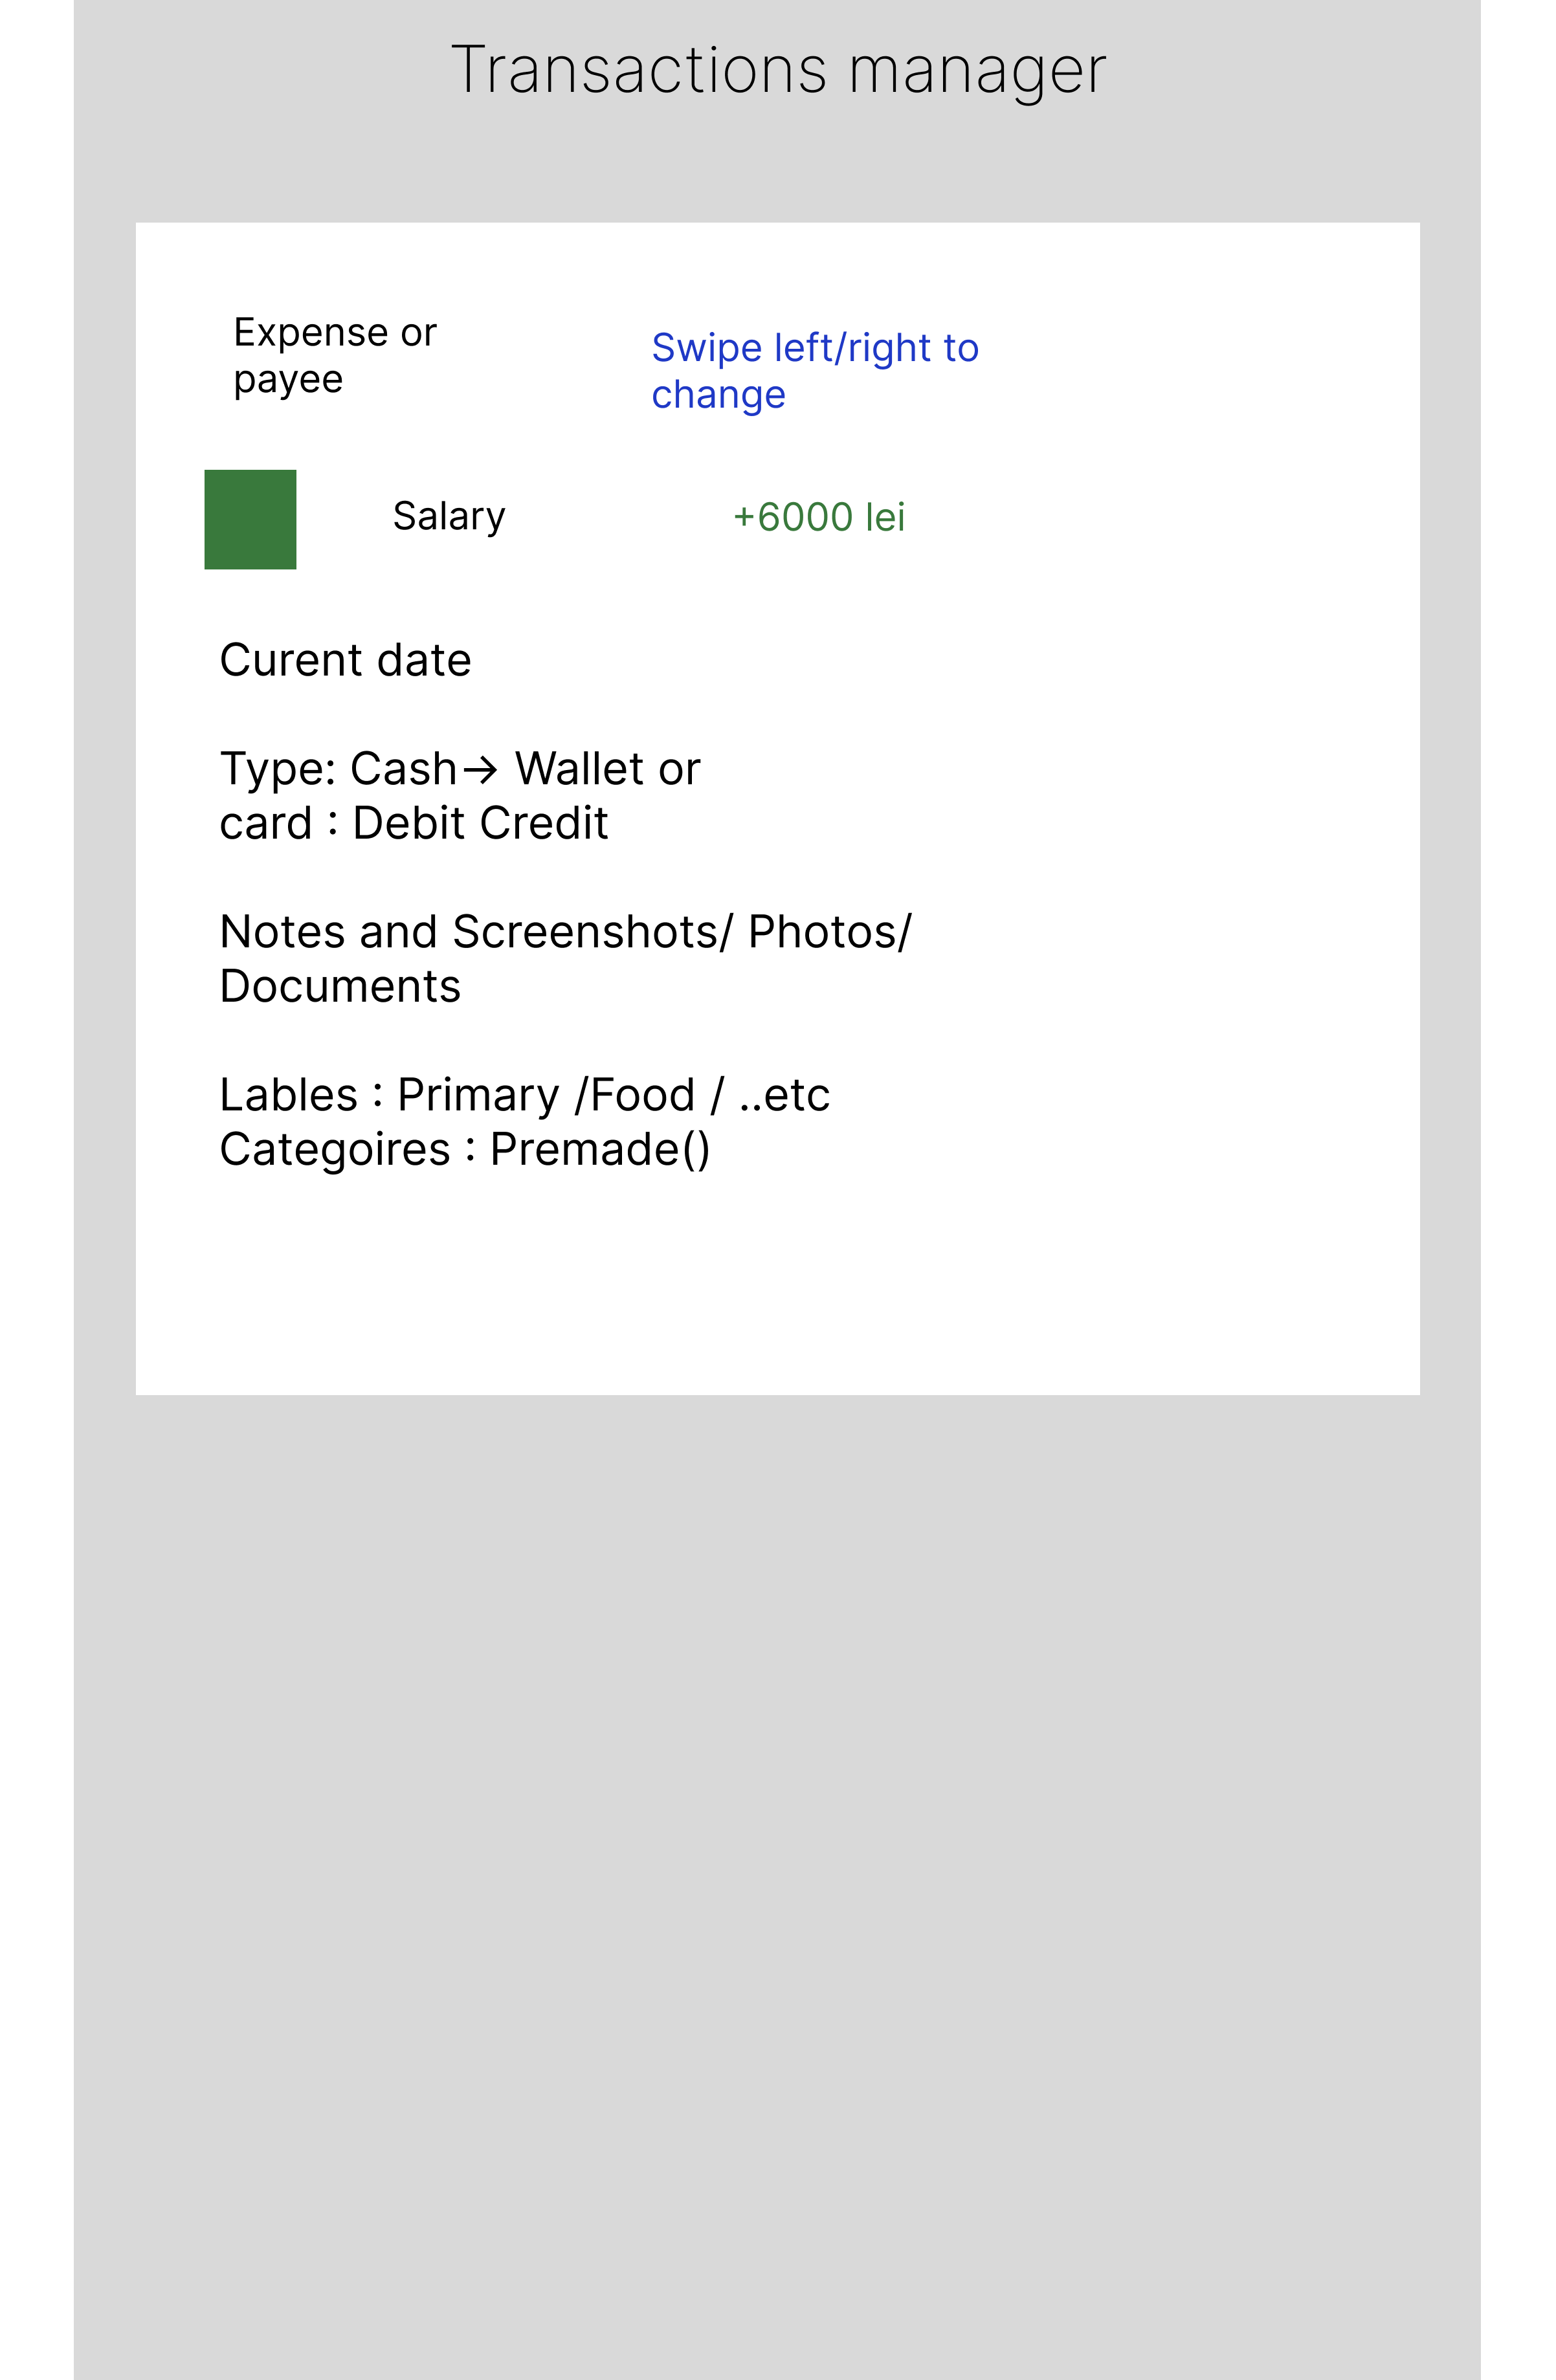
\includegraphics[width=\textwidth]{Graphics/Design/TM_I.png}
    \caption{Income Transaction Screen}
    \label{fig:image3}
  \end{minipage}
\end{figure}



After this short brainstorming session, a design layout in Figma was created. Upon reflection, it was realized that the color composition appeared to be uneven. The color palette used in the design was diverse and did not align with the simplistic and easy-to-use interface envisioned.

% \begin{figure}[htbp]
%   \centering
%   \begin{minipage}[b]{0.32\textwidth}
%     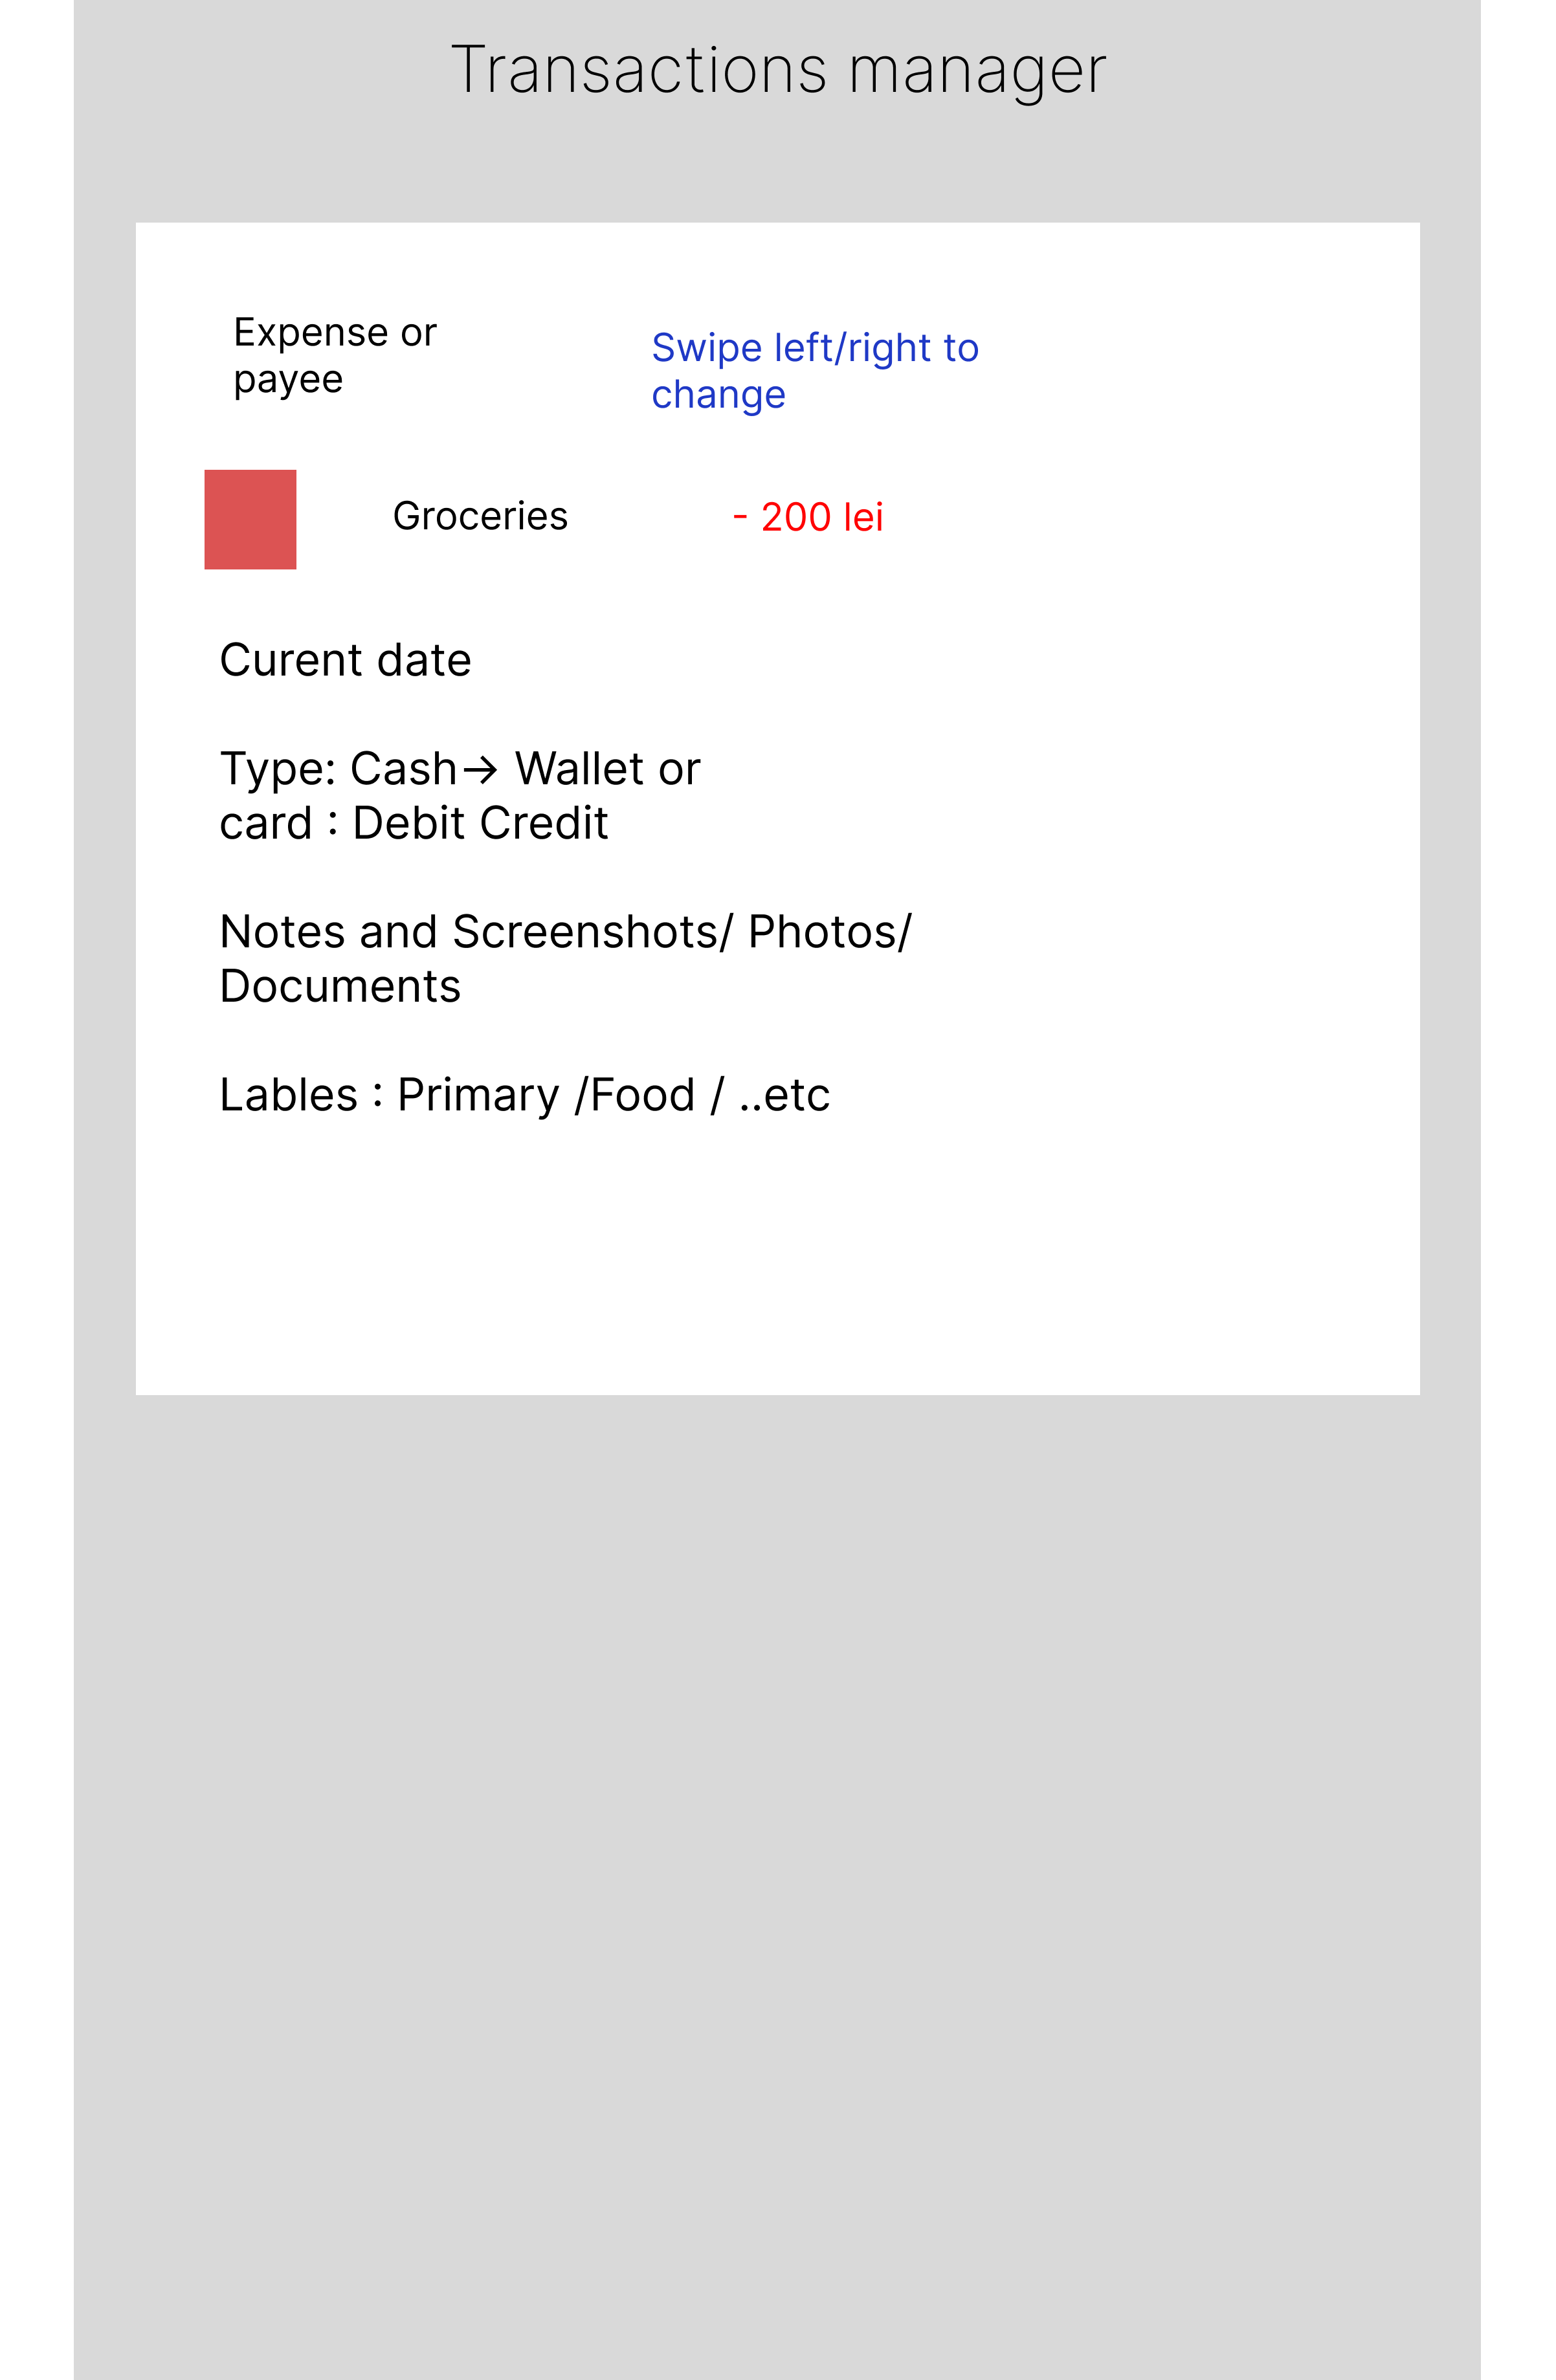
\includegraphics[width=\textwidth]{Graphics/Design/TM_E.png}
%     \caption{Blue Coins main menu 1.}
%     \label{fig:image1}
%   \end{minipage}
%   \hfill
%   \begin{minipage}[b]{0.32\textwidth}
%     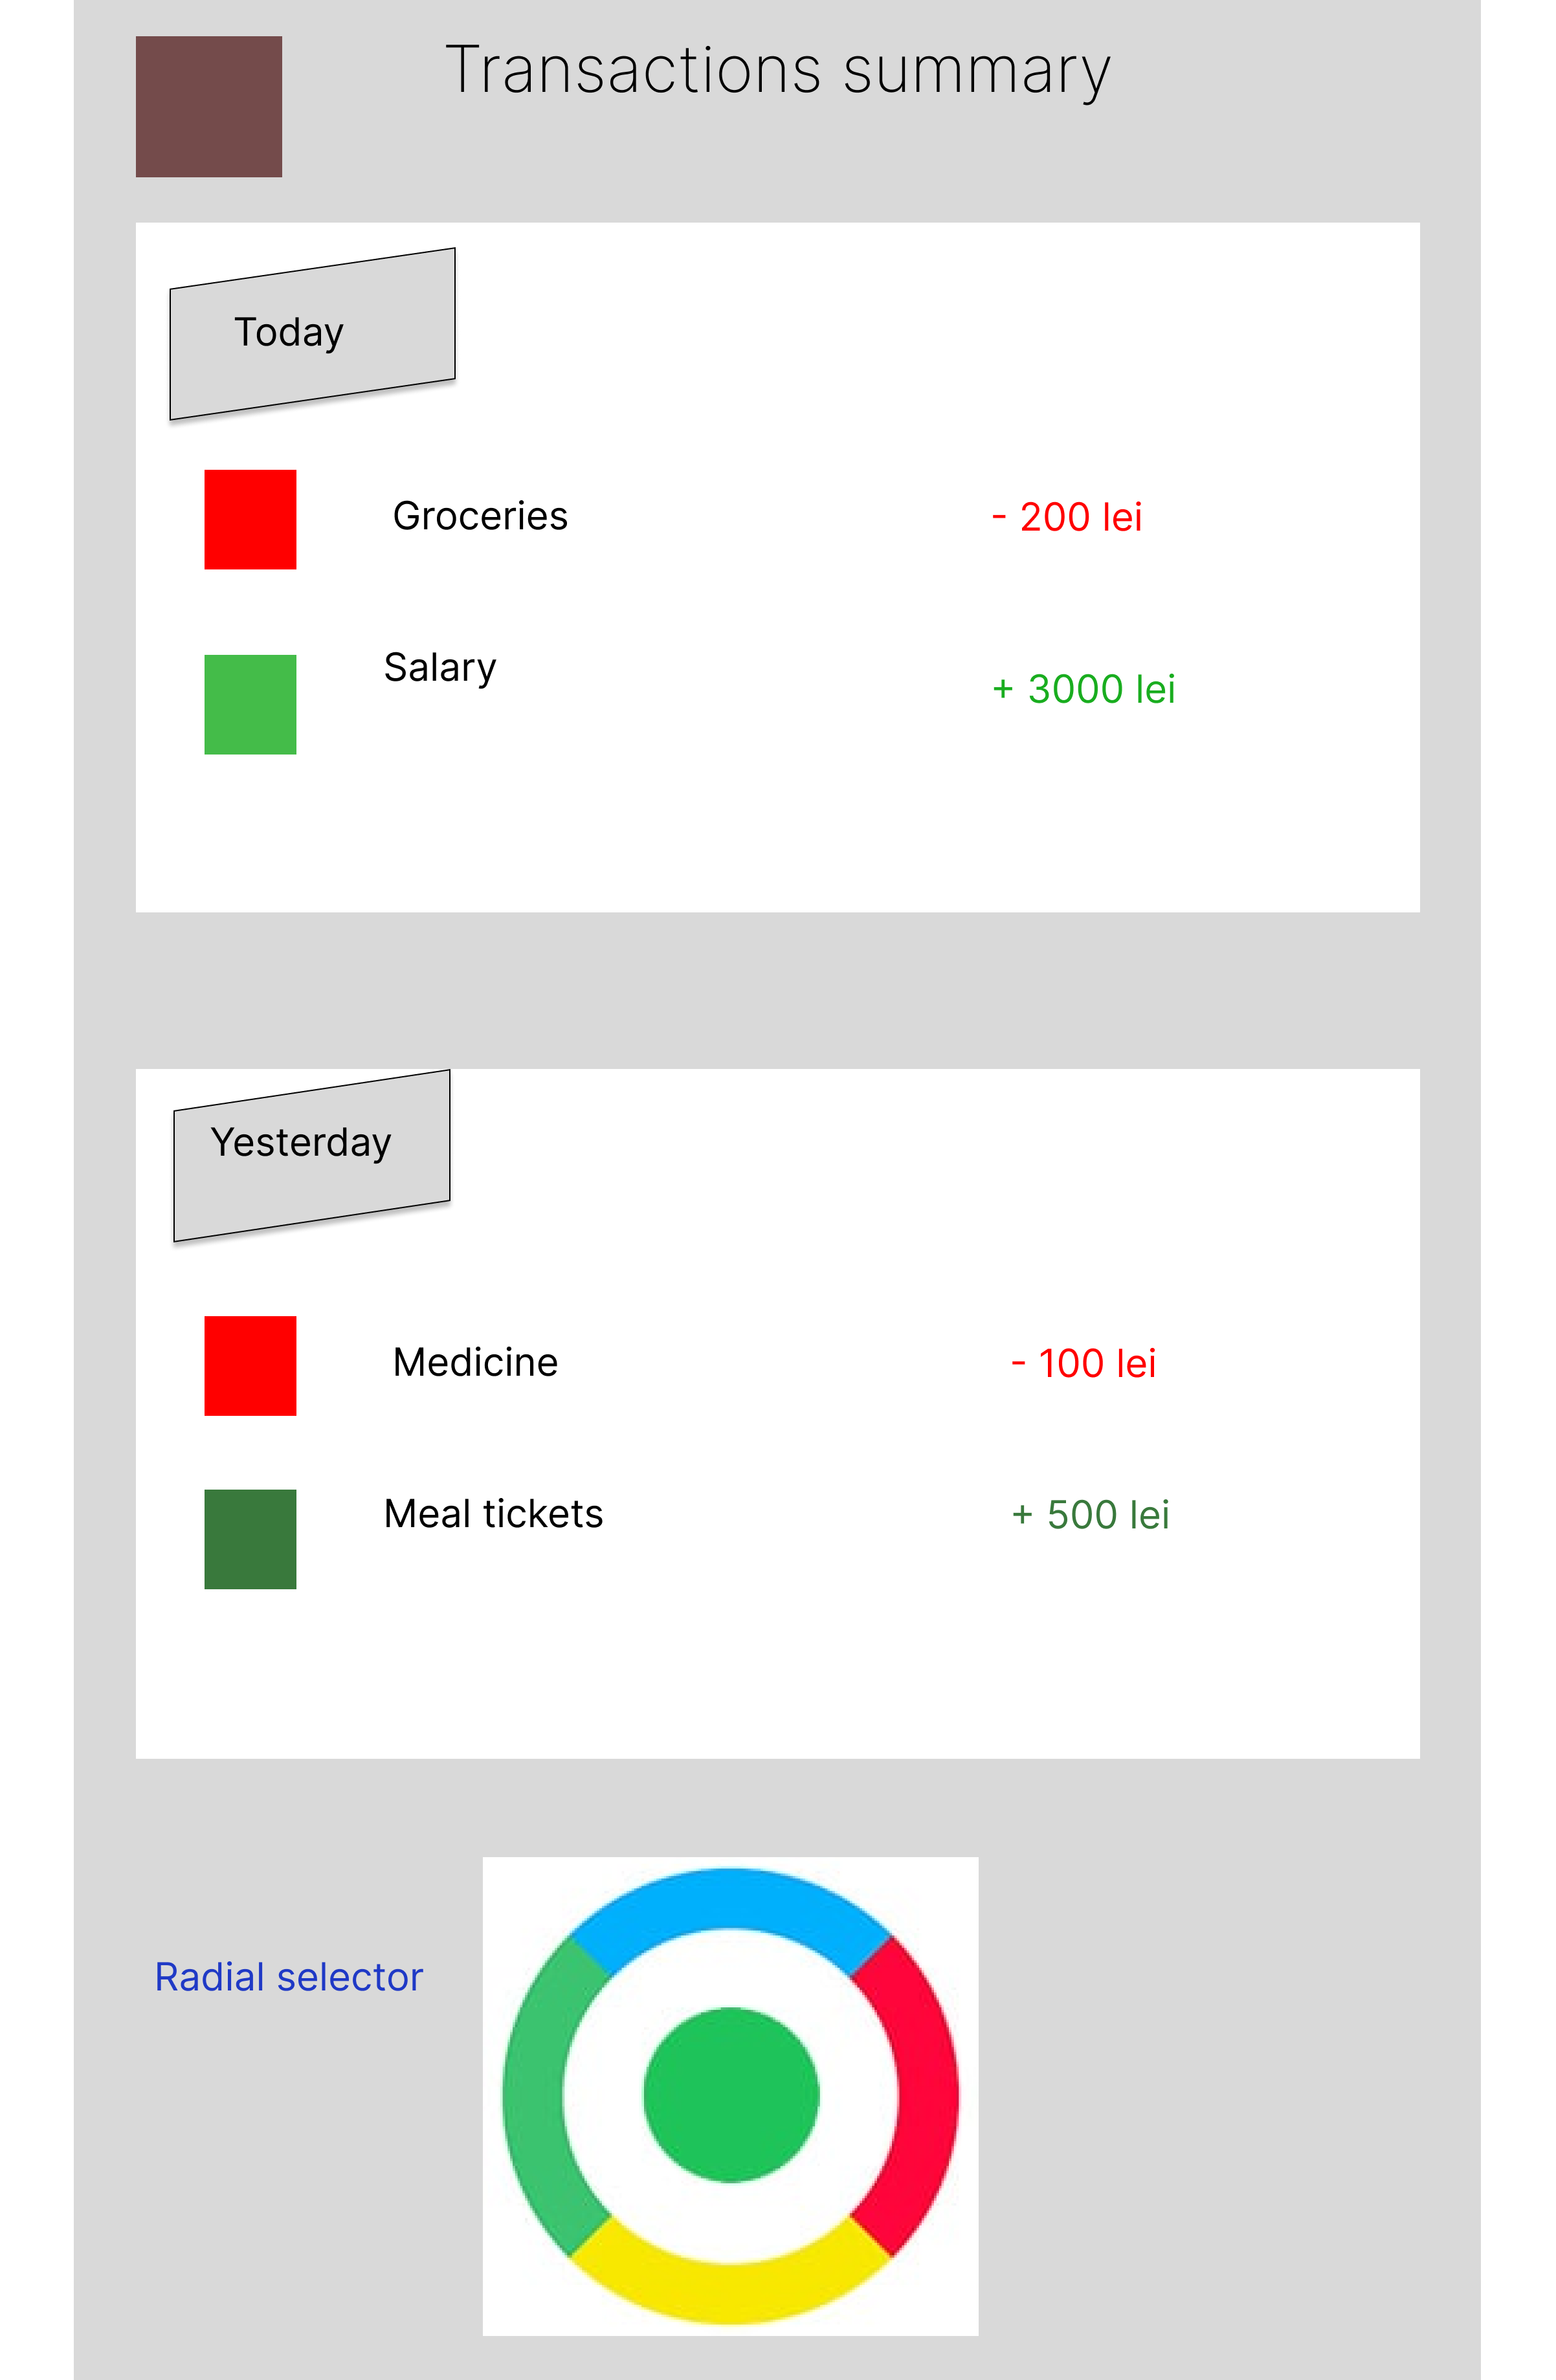
\includegraphics[width=\textwidth]{Graphics/Design/TM_Menu.png }
%     \caption{Blue coins Dark main menu.}
%     \label{fig:image2}
%   \end{minipage}
%   \hfill
%   \begin{minipage}[b]{0.32\textwidth}
%     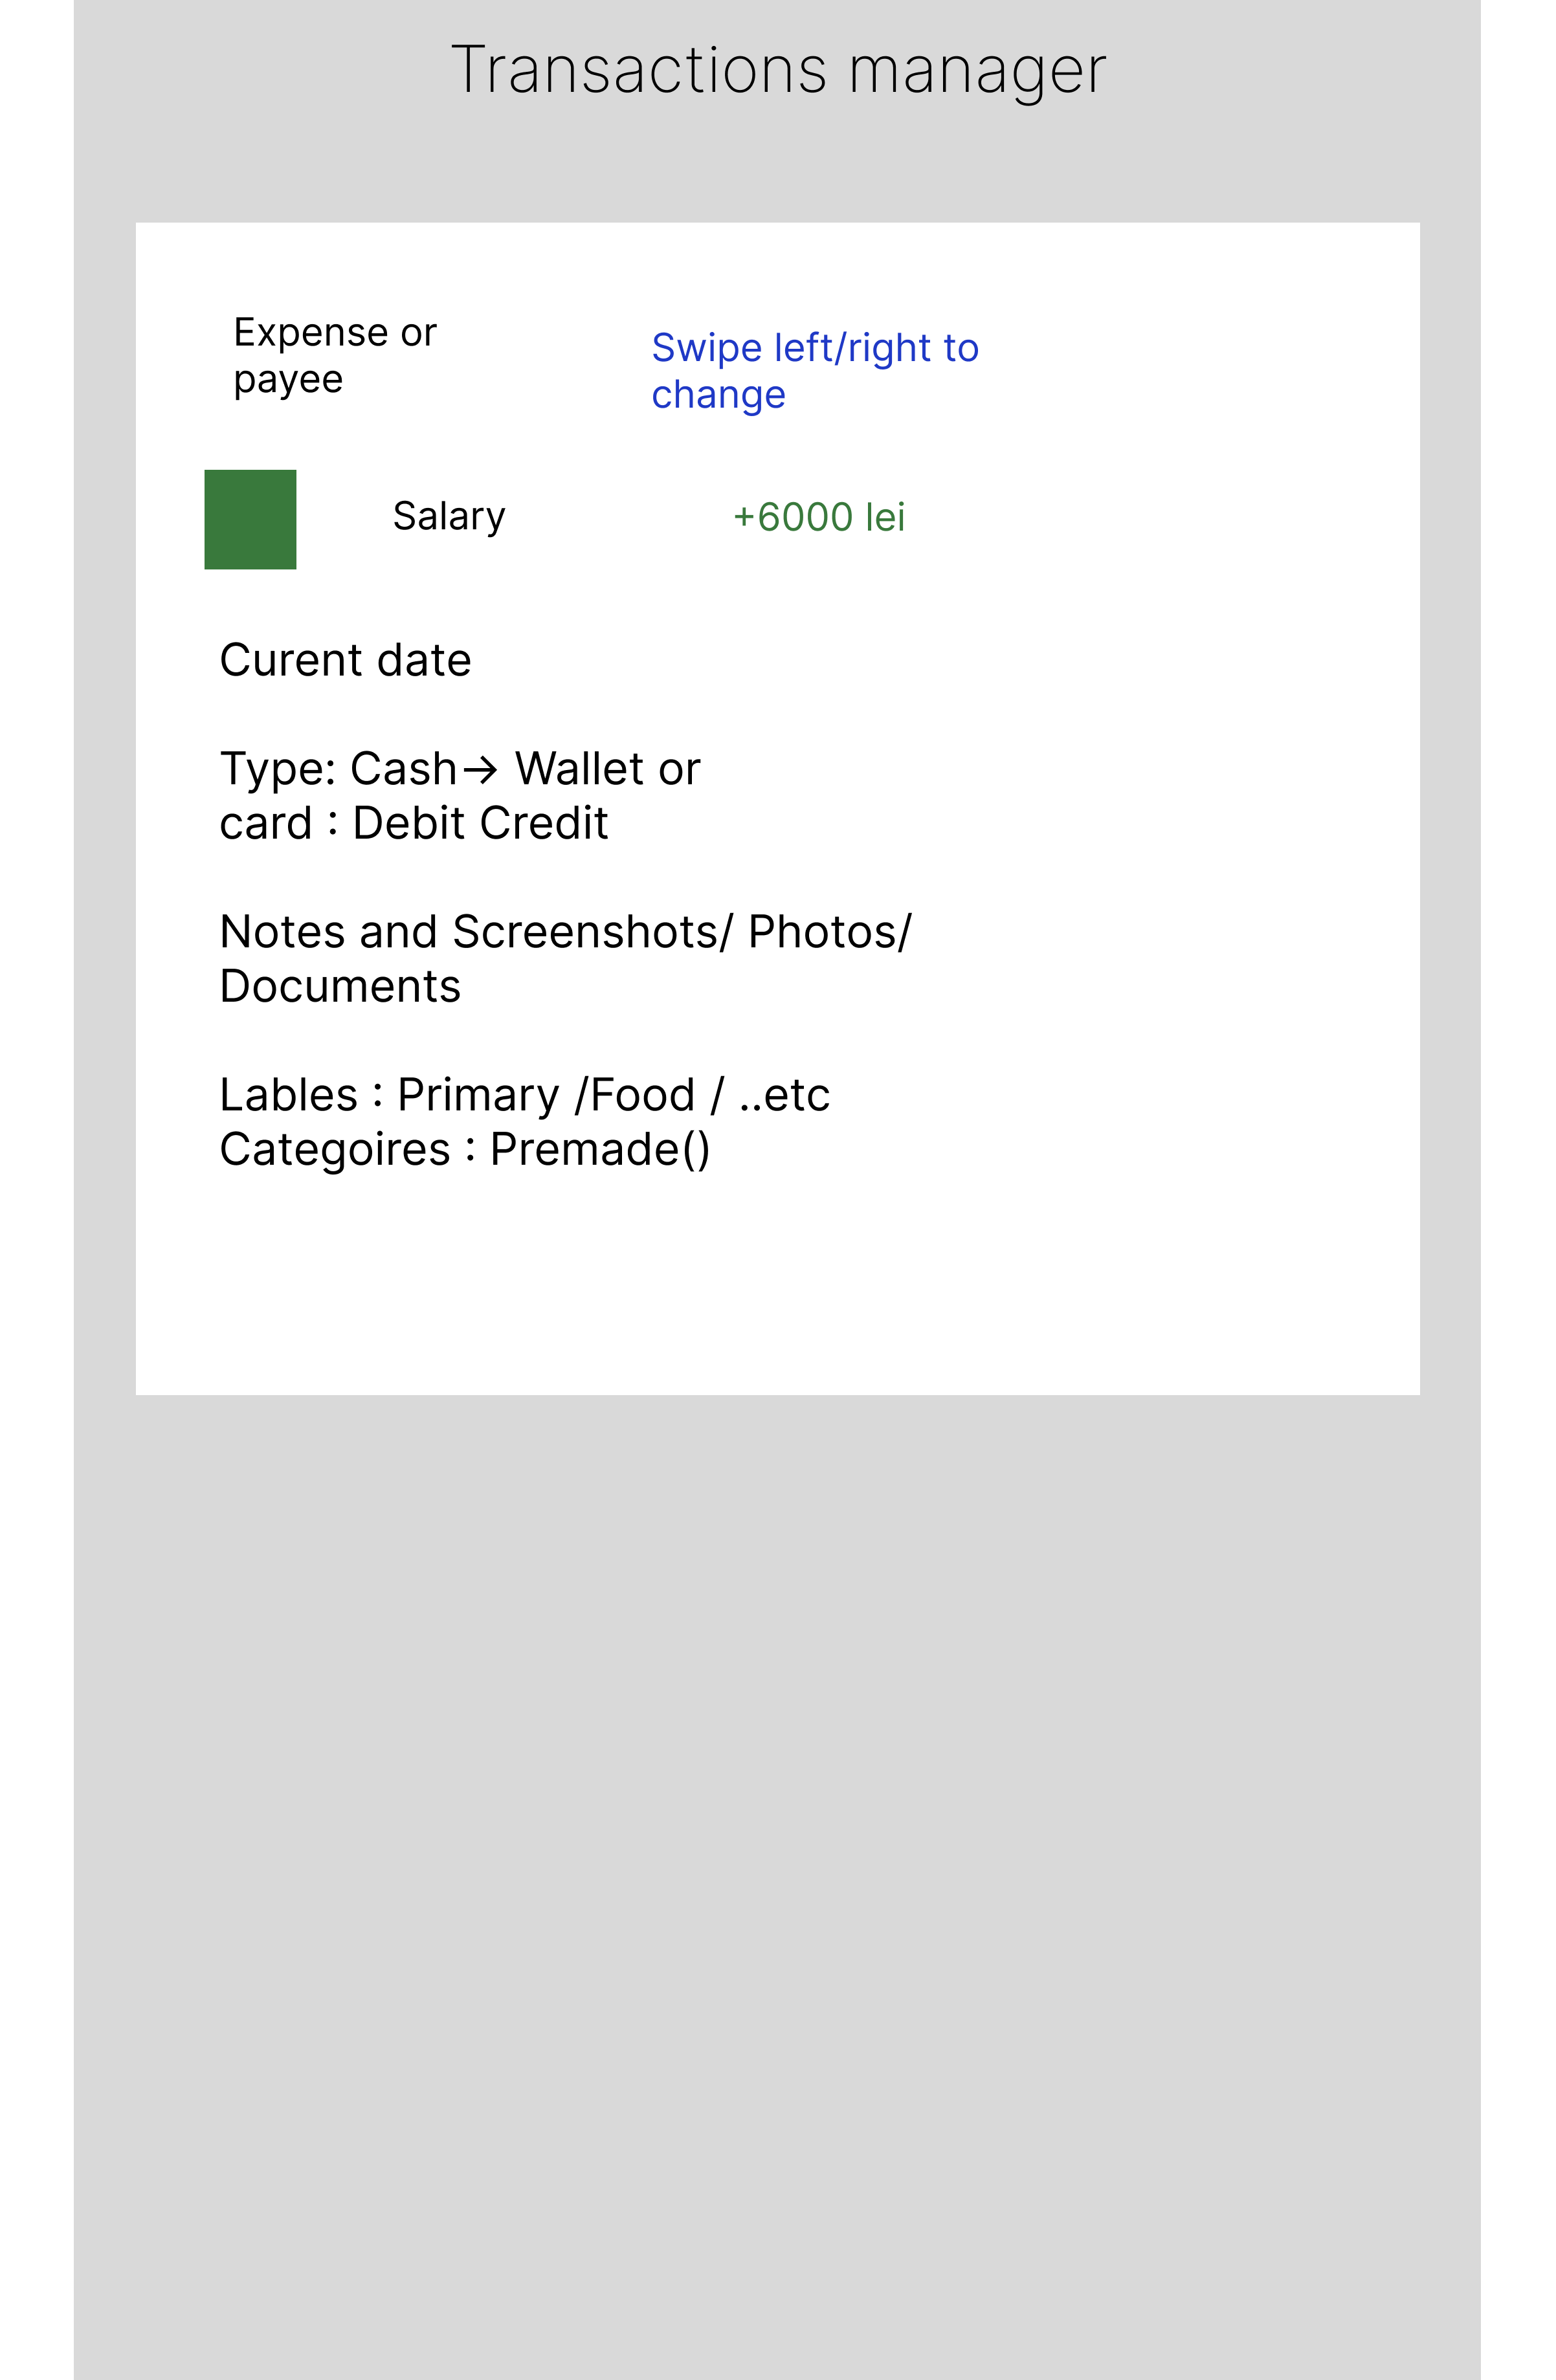
\includegraphics[width=\textwidth]{Graphics/Design/TM_I.png}
%     \caption{Blue Coins Yellow main menu.}
%     \label{fig:image3}
%   \end{minipage}
% \end{figure}

\subsection{Second Design Iteration}


\textit{Purple} was chosen as the primary color for the transaction menu, taking into consideration factors such as uniqueness and elegance. It was believed that \textit{purple} could add a touch of \textit{luxury, creativity, and sophistication} to the app, which is not commonly seen in financial apps.

To ensure cohesiveness, different shades of \textit{purple} were utilized to represent various transaction types. A lighter shade of \textit{purple} was assigned to income transactions, while a darker shade was designated for expenses. Additionally, the author considered using other colors, such as \textit{green} or \textit{blue}, to represent additional transaction types like savings or investing.

The author made sure that the chosen \textit{purple} color was easily distinguishable from other colors used in the app and did not clash with other elements on the screen. To achieve this, a color wheel or palette generator was employed to find complementary colors to use alongside \textit{purple}.

As part of the design process, a simple Profile Page was created for the application. The author found that the new design was a better fit for their desired simplistic approach and aligned well with their overall vision.


In this second design iteration, the application's color scheme was carefully chosen to create a visually appealing and cohesive user interface. The following images showcase various perennially designed templates that were incorporated into the application, enhancing its overall aesthetic and user experience. These design templates provide consistent styling and layout for key components such as buttons, forms, and cards, creating a unified and professional look throughout the application. 

\begin{figure}[htbp]
  \centering
  \begin{minipage}[b]{0.23\textwidth}
    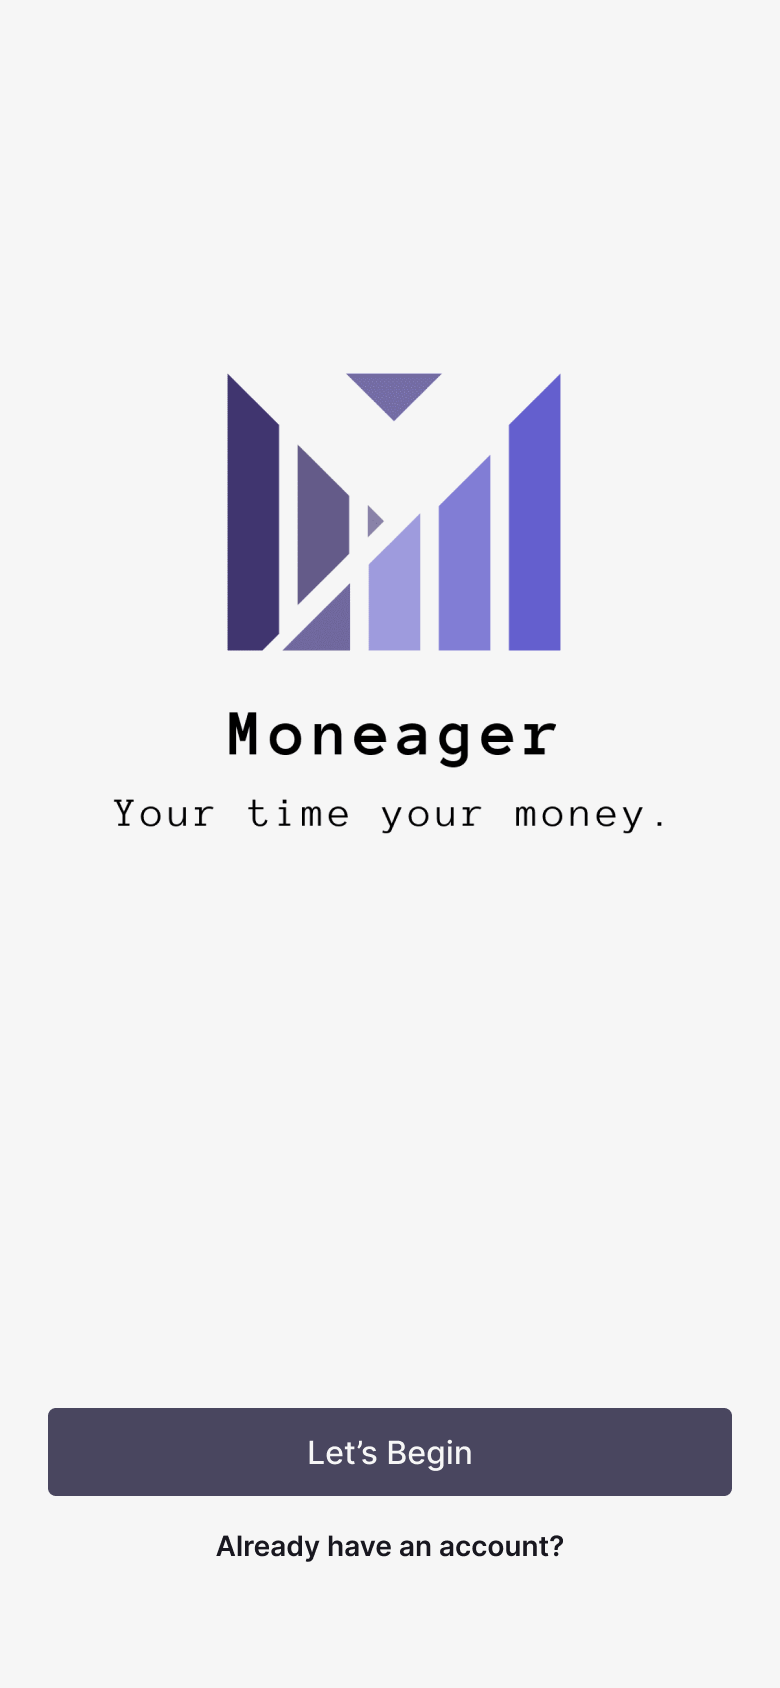
\includegraphics[width=\textwidth]{Graphics/FinalDesigns/FirstMenu.png}
    \caption{First Menu}
    \label{fig:image1}
  \end{minipage}
  \hfill
  \begin{minipage}[b]{0.23\textwidth}
    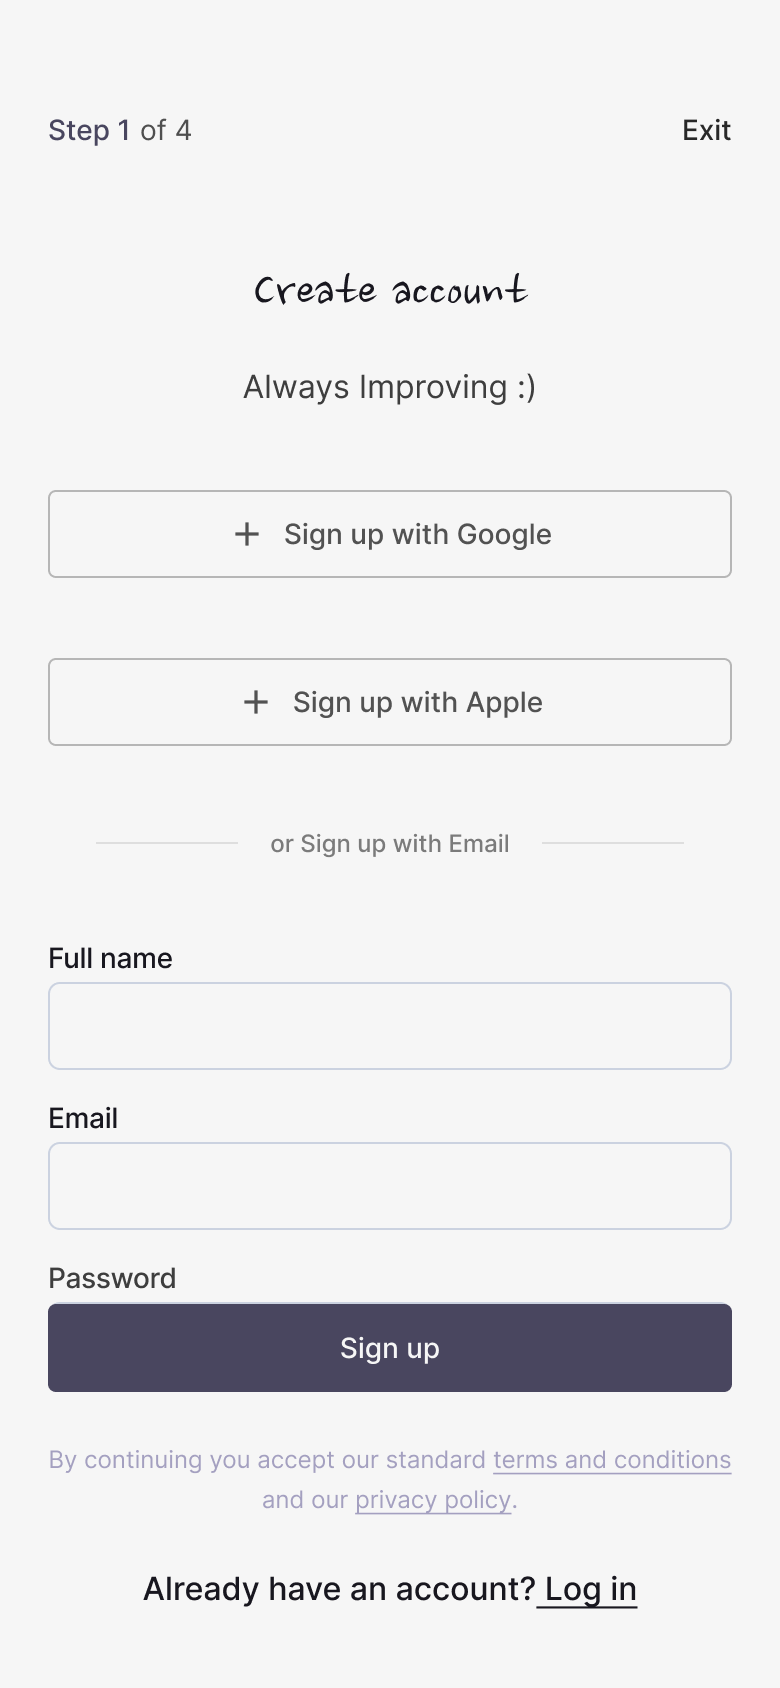
\includegraphics[width=\textwidth]{Graphics/FinalDesigns/LoginScreen.png}
    \caption{Login Screen}
    \label{fig:image2}
  \end{minipage}
\end{figure}


\newpage


